\documentclass[a4paper,10pt]{article}

\usepackage[T1]{fontenc}
\usepackage[utf8]{inputenc}
\usepackage{lmodern}
\usepackage[margin=2.5cm]{geometry}
\usepackage{amsmath,amssymb}
\usepackage{graphicx}
\usepackage{booktabs}
\usepackage{array}
\usepackage{longtable}
\usepackage{xcolor}
\usepackage{listings}
\usepackage{caption}
\usepackage{xurl}
\usepackage[hidelinks]{hyperref}

\captionsetup{font=small,labelfont=bf}
\setlength{\emergencystretch}{3em}
\setlength{\parindent}{0pt}
\setlength{\parskip}{0.5em}

\DeclareRobustCommand{\code}[1]{\path{#1}}
\newcommand{\degC}{\,$^\circ$C}

\definecolor{codebg}{HTML}{F5F5F3}
\definecolor{codekw}{HTML}{1C5CAB}
\definecolor{codecm}{HTML}{52514E}
\lstset{language=Python, basicstyle=\ttfamily\footnotesize, backgroundcolor=\color{codebg},
  keywordstyle=\color{codekw}, commentstyle=\color{codecm}\itshape, stringstyle=\color{black},
  frame=none, breaklines=true, columns=fullflexible, showstringspaces=false,
  xleftmargin=0.5em, xrightmargin=0.5em, aboveskip=0.6em, belowskip=0.6em}

\title{PhlyGreen Technical Manual: Battery}
\author{PhlyGreen development team, Sapienza University of Rome}
\date{Code state: November 2026, branch \texttt{main}}

\begin{document}
\maketitle

\begin{abstract}
\noindent This manual documents the battery in PhlyGreen. It covers the two battery models
(Class~I and Class~II), the cell-level electro-thermal model and its equations, the sizing of
the pack inside the take-off-weight loop, the coupling with the powertrain, the ground segments,
the state of health and the post-design ageing analysis. Every equation is traced to the
function that implements it, and every number is produced by the scripts in
\code{manuals/battery/scripts/}. The manual is written for the lead developer and for MSc
students who need to modify or extend the model.
\end{abstract}

\tableofcontents
\clearpage

%======================================================================
\section{Scope and conventions}
\label{sec:scope}
%======================================================================

This section states where the battery enters PhlyGreen and fixes the notation used in the rest
of the manual.

\subsection{Where the battery appears}

The battery is a subsystem of the \texttt{Aircraft} mediator (\code{trunk/PhlyGreen/Aircraft.py}).
The class is \code{Battery} in \code{trunk/PhlyGreen/Systems/Battery/Battery.py}; the factory
\code{pg.build_aircraft()} wires it like every other subsystem. Three aircraft configurations
carry a battery. Table~\ref{tab:configs} lists them with the mission and weight methods that
handle the battery.

\begin{table}[h]
\centering\small
\caption{Configurations with a battery and the methods that size it.}
\label{tab:configs}
\begin{tabular}{@{}p{3.4cm}p{1.2cm}p{5.6cm}p{4.2cm}@{}}
\toprule
Configuration & Battery & Mission method (\code{Mission/Mission.py}) & Battery mass (\code{Weight/Weight.py})\\
\midrule
\texttt{'Hybrid'}, \texttt{'Parallel'} or \texttt{'Serial'} & Class I & \code{HybridConfigurationClassI} & \code{Weight.Hybrid}, three candidates\\
\texttt{'Hybrid'}, \texttt{'Parallel'} or \texttt{'Serial'} & Class II & \code{HybridConfigurationClassII} & \code{Weight.Hybrid}, \code{pack_weight}\\
\texttt{'Hybrid'}, \texttt{'Serial'}, with \texttt{gt\_rated\_power} & Class I & \code{SerialRangeExtenderConfiguration} & \code{Weight.Hybrid}, three candidates on the buffer swing\\
\texttt{'FuelCellBattery'} & Class I & \code{FuelCellBatteryConfiguration} & \code{Weight.FuelCellBattery}, two candidates\\
\texttt{'FuelCellBattery'} & Class II & \code{FuelCellBatteryConfigurationClassII} & \code{Weight.FuelCellBattery}, \code{pack_weight}\\
\bottomrule
\end{tabular}
\end{table}

The dispatch is in \code{Mission._fly_configuration}. A serial hybrid with a
\texttt{'GT Rated Power'} input is always flown as a range extender. The range extender reads
no cell model, so it is a Class-I path regardless of \texttt{CellInput}. The fuel cell stack,
its thermal management and the hydrogen tank are outside the scope of this manual. They are
documented in the companion manuals ``PhlyGreen Technical Manual: Fuel Cell'' and ``PhlyGreen
Technical Manual: Thermal Management''. This manual covers the battery cooling mass term,
which is separate from the fuel-cell thermal-management system.

\subsection{The supplied power ratio}
\label{sec:phi}

The battery share of the power is set by the supplied power ratio $\varphi$. Each mission
segment carries a \texttt{'Supplied Power Ratio'} block, either a constant \texttt{phi} or a
linear ramp from \texttt{phi\_start} to \texttt{phi\_end} in time. \code{Profile.DefineMission}
builds the schedule and \code{Profile.SuppliedPowerRatio(t)} interpolates it linearly inside
each segment. A break time belongs to the segment that starts there (\code{numpy.searchsorted},
as in \code{Profile.Altitude} and \code{Profile.Velocity}), so each segment is integrated with its
own $\varphi$ from its first point. The \texttt{'Takeoff'} stage carries only a constant \texttt{phi}, the take-off
ratio $\varphi_{TO}$. It is stored as \code{Profile.SPW[0]} and read by
\code{Mission._takeoff_phi}. The taxi ratio $\varphi_{taxi}$ is the input
\code{MissionConfig.taxi_phi}; it defaults to $\varphi_{TO}$ (\code{Mission._taxi_phi}).

The meaning of $\varphi$ is not the same in all configurations; \code{docs/user-guide/mission.md}
states it as well. We state it precisely because it changes the numbers.
\begin{itemize}
\item In \texttt{'Hybrid'}, $\varphi$ enters the powertrain graph as the split equation
  $\varphi P_f + (\varphi-1) P_{bat} = 0$ (\code{graph.PowertrainGraph.split}). Here $P_f$ is
  the fuel chemical power and $P_{bat}$ the battery terminal power. Therefore
  \begin{equation}
  \varphi = \frac{P_{bat}}{P_f + P_{bat}},
  \label{eq:phi-hybrid}
  \end{equation}
  that is, the battery fraction of the total \emph{supplied} power (chemical plus electrical).
  Because the gas-turbine efficiency is low, a given $\varphi$ corresponds to a much smaller
  battery fraction of the shaft power.
\item In \texttt{'FuelCellBattery'}, $\varphi$ is the battery fraction of the
  \emph{propulsive} power $P_p$. The battery delivers $\varphi P_p$ and the fuel cell
  $(1-\varphi)P_p$ (\code{Mission.FuelCellBatteryConfiguration}).
\item The serial range extender ignores $\varphi$. The turbine runs at its rated power and the
  battery covers the difference (Section~\ref{sec:re}).
\end{itemize}

\subsection{Reference configurations}
\label{sec:baselines}

All numbers in this manual come from the baselines in \code{trunk/examples/common.py}:
\begin{itemize}
\item \code{hybrid_config('I')} and \code{hybrid_config('II')}: an ATR-like parallel hybrid
  (750~nm design range, 220~nm diversion, 4560~kg payload). The cruise $\varphi$ ramps from 0
  to 0.5; all other segments and the take-off have $\varphi=0$. The Class-I battery has
  1500~Wh/kg, 8000~W/kg and $\mathrm{SOC}_{min}=0.2$. The Class-II battery uses the
  \texttt{'Finger-Cell-Thermal'} cell rescaled to the same specific energy and power, an
  800~V pack, 25\degC\ initial temperature and a 50\degC\ ceiling.
\item \code{fuelcell_battery_config(cruise_phi)}: the hydrogen fuel-cell aircraft with a
  Class-I battery of 250~Wh/kg, 1500~W/kg and 0.8 usable SOC.
\end{itemize}
These specific energies are scenario inputs of the examples. The 1500~Wh/kg value is far
above present cells; it is the example default, not a recommendation. The scripts
\code{fig_cell.py}, \code{fig_class_ii_mission.py} and \code{fig_sizing_studies.py} change
only the parameters stated in each figure caption. They write the quoted numbers to
\code{manuals/battery/data/*.json}.

%======================================================================
\section{Class I battery model}
\label{sec:classI}
%======================================================================

The Class-I model treats the pack as a mass with a fixed specific energy and a fixed specific
power. It has no voltage, no current and no temperature.

\subsection{Gas-turbine hybrid}

\code{Battery.SetInput} reads three keys of \texttt{CellInput}: \texttt{'SpecificEnergy'} $e_b$ [Wh/kg],
\texttt{'SpecificPower'} $p_b$ [W/kg] and \texttt{'Minimum SOC'}. It
stores $E_{bat}=3600\,e_b$ [J/kg] as \code{Battery.Ebat} and $p_b$ as \code{Battery.pbat}. The
mission (\code{Mission.HybridConfigurationClassI}) integrates three states,
\begin{equation}
\frac{dE_f}{dt} = P_p\,\Pi_0,\qquad
\frac{dE_{b}}{dt} = P_p\,\Pi_5,\qquad
\frac{d\beta}{dt} = -\frac{P_p\,\Pi_0}{e_f\,W_{TO}},
\label{eq:classI-ode}
\end{equation}
where $P_p(\beta,t)$ is the propulsive power from \code{Performance.PoWTO}, $\beta=W/W_{TO}$
the mass fraction, $e_f$ the fuel specific energy, and $\Pi_k$ the power ratios returned by
\code{Powertrain.Hybrid} (Section~\ref{sec:powertrain}). $\Pi_5=P_{bat}/P_p$ is the battery
terminal power per unit propulsive power. The integration runs segment by segment with
\code{scipy.integrate.solve_ivp} (BDF, \code{rtol=1e-5}).

\code{Weight.Hybrid} takes the battery mass as the largest of three candidates:
\begin{equation}
W_{bat} = \max\left(\frac{E_b}{(1-\mathrm{SOC}_{min})\,E_{bat}},\;
\frac{P_{bat,max}}{p_b},\;\frac{P_{bat,TO}}{p_b}\right).
\label{eq:classI-mass}
\end{equation}
$E_b$ is the battery energy of the mission plus the ground segments
(Section~\ref{sec:ground}). $P_{bat,max}$ is \code{Mission.Max_PBat}, the peak battery terminal
power over the profile, the taxi and the take-off run. $P_{bat,TO}$ is \code{Mission.TO_PBat},
the battery share of the worst-case take-off or one-engine-inoperative (OEI) power
(\code{Mission._worst_case_propulsive_power}) at $\varphi_{TO}$. The index of the binding
candidate is stored in \code{Weight.WBatidx} (0 energy, 1 mission power, 2 take-off power).

\subsection{Fuel-cell + battery}

The \texttt{'FuelCellBattery'} configuration without a \texttt{CellInput} uses its own Class-I
battery, defined in \texttt{EnergyInput}. \code{Weight.FuelCellBattery} computes
\begin{equation}
W_{bat} = \max\left(\frac{E_b/3600}{e_b\,c\,\sigma_u},\; \frac{P_{bat,max}\,r}{p_b}\right),
\label{eq:fcb-mass}
\end{equation}
with $e_b$ = \texttt{'Battery Specific Energy'} (default 250~Wh/kg), $p_b$ =
\texttt{'Battery Specific Power'} (default 1500~W/kg), $\sigma_u$ = \texttt{'Battery Usable
SOC'} (default 0.8), and the state-of-health factors $c$ and $r$ of Section~\ref{sec:soh}.
Two points matter. First, the usable fraction is an
explicit input $\sigma_u$ instead of $1-\mathrm{SOC}_{min}$. Second, the propulsive share of the battery is $\varphi P_p$, and its terminal power is
$\varphi P_p/\eta_{el}$ with $\eta_{el}=\eta_{EM}\eta_{PM}\eta_{GB}\eta_{prop}$
(\code{Mission._fc_battery_eta_elec}, the same chain as the fuel-cell branch). The battery energy
$E_b$, the peak power $P_{bat,max}$ and the take-off power $P_{bat,TO}$ are all terminal
quantities (\code{Mission.FuelCellBatteryConfiguration}), as in \code{Weight.Hybrid}.

On \code{fuelcell_battery_config(0.15)} the battery draws 1066.3~kWh. The energy candidate is
5331.3~kg and the power candidate 324.2~kg, so the pack is energy limited, and
$W_{TO}=40\,103$~kg.

\subsection{Energy- and power-limited packs}

Figure~\ref{fig:classI} shows the three candidates of Eq.~\eqref{eq:classI-mass} on
\code{hybrid_config('I')}. In panel~(a) the battery flies only in cruise. The energy
candidate binds everywhere: at a constant cruise $\varphi=0.5$ it is 2590.3~kg, while the
power candidate is 177.4~kg. In panel~(b) the battery flies only the ground segments and the
take-off. Here the power candidates bind: at $\varphi_{TO}=0.3$ the pack is 258.3~kg against an
energy candidate of 72.3~kg. The mission-power and take-off-power curves coincide in panel~(b).
The reason is that the take-off run is flown at the full take-off power, and the take-off power
is the larger of the take-off and OEI cases, so $P_{bat,max}=P_{bat,TO}$.

\begin{figure}[t]
\centering
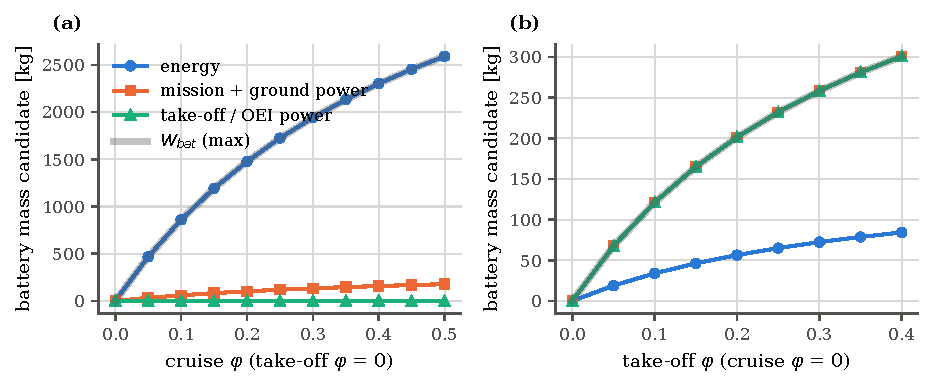
\includegraphics[width=\textwidth]{figures/fig_class_i_sizing.pdf}
\caption{Class-I battery mass candidates of Eq.~\eqref{eq:classI-mass} at the converged design
of \code{hybrid_config('I')}. (a)~Constant cruise $\varphi$, no take-off battery. (b)~Take-off
battery ($\varphi_{TO}$, and $\varphi_{taxi}=\varphi_{TO}$ by default), $\varphi=0$ in flight.
The grey band is the selected mass $W_{bat}$. Script: \code{fig_sizing_studies.py}.}
\label{fig:classI}
\end{figure}

A power-limited pack has a large effect on the rest of the aircraft. At $\varphi_{TO}=0.3$ the
electric motor (413.2~kg) and the power-management and distribution unit (PMAD, 206.6~kg) weigh
more than the battery, because both are sized on the battery power (Section~\ref{sec:motor}).

%======================================================================
\section{Class II cell model}
\label{sec:classII-theory}
%======================================================================

The Class-II model represents one cell with a temperature-dependent Shepherd--Tremblay voltage
law and a lumped thermal balance. A pack of $S$ cells in series and $P$ in parallel is built
from it, and every cell carries the same current and power.

\subsection{Voltage model}

The cell terminal voltage is implemented in \code{Battery._voltageModel}:
\begin{equation}
V(i_t, i, T) = E_0(T) - (i + i_t)\,K(T)\,\frac{Q(T)}{Q(T)-i_t} + A\,e^{-B\,i_t} - i\,R(T).
\label{eq:shepherd}
\end{equation}
The symbols are:
\begin{itemize}
\item $i$ [A], the cell current (positive in discharge);
\item $i_t$ [Ah], the charge already drawn from the cell (the current integral);
\item $E_0$ [V], the voltage constant (\texttt{'Voltage Constant'});
\item $K$ [V/Ah], the polarization constant (\texttt{'Polarization Constant'}). It multiplies
  both the polarization voltage $K\,i_t\,Q/(Q-i_t)$ and the polarization resistance term
  $K\,i\,Q/(Q-i_t)$;
\item $Q$ [Ah], the cell capacity (\texttt{'Cell Capacity'});
\item $A$ [V] and $B$ [Ah$^{-1}$], the amplitude and inverse charge constant of the exponential
  zone (\texttt{'Exp Amplitude'}, \texttt{'Exp Time constant'});
\item $R$ [$\Omega$], the ohmic internal resistance (\texttt{'Internal Resistance'}).
\end{itemize}
The open-circuit voltage is $V_{oc}(i_t)=V(i_t,0)$ (\code{Battery.cell_Voc}). The model is the
thermal-corrected form referenced in \code{Cell_Models.py} (DOI 10.1109/TIE.2016.2618363),
and \code{docs/user-guide/battery.md} lists the Shepherd (1965) and Tremblay and Dessaint (2007)
papers as its origin. The maximum cell voltage is defined as $V_{max}=E_0+A$
(\code{SetInput}). It is used only to choose the number of cells in series.

The state of charge is the charge balance against the nominal capacity $Q_0$ (\code{Battery.SOC}):
\begin{equation}
\mathrm{SOC} = 1 - \frac{i_t}{Q_0}.
\label{eq:soc}
\end{equation}
Note that the SOC uses the reference capacity $Q_0$ (\code{cell_capacity}), while the voltage
uses the temperature-corrected $Q(T)$ of Eq.~\eqref{eq:temperature}.

\subsection{Temperature dependence}

The four parameters that depend on temperature are properties of the class
(\code{Battery.E0}, \code{Q}, \code{K}, \code{R}):
\begin{equation}
\begin{aligned}
E_0(T) &= E_{0,ref} + \frac{\partial E}{\partial T}\,(T-T_{ref}), &
Q(T) &= Q_0 + \frac{\partial Q}{\partial T}\,(T-T_{ref}),\\
K(T) &= K_{ref}\exp\!\left[\alpha_K\left(\frac{1}{T}-\frac{1}{T_{ref}}\right)\right], &
R(T) &= R_{ref}\exp\!\left[\alpha_R\left(\frac{1}{T}-\frac{1}{T_{ref}}\right)\right].
\end{aligned}
\label{eq:temperature}
\end{equation}
$\partial E/\partial T$ [V/K] is the \texttt{'Voltage Thermal Slope'}, $\partial Q/\partial T$
[Ah/K] the \texttt{'Capacity Thermal Slope'}, and $\alpha_K$, $\alpha_R$ [K] the
\texttt{'Polarization Arrhenius Constant'} and \texttt{'Resistance Arrhenius Constant'}. The
Arrhenius constants are activation temperatures, in K. $A$ and $B$ do not depend on temperature.

\subsection{Cell database}

Table~\ref{tab:cells} lists the two entries of \code{Cell_Models.py}. The comments in the file
state their origin: \texttt{'ThermalModel-Cell'} is the 120-cell reference pack of the cited
paper, with mass and geometry taken from the Molicel INR-21700-P50B datasheet;
\texttt{'Finger-Cell-Thermal'} combines values of that paper with the same datasheet. The
reference temperature is $273.15+23=296.15$~K (23\degC). The capacity thermal slope of the
finger cell is that of the reference pack scaled to its capacity, $0.1766\cdot6/42.82$~Ah/K, so
both have the same relative slope of 0.41~\%/K.

\begin{table}[h]
\centering\small
\caption{Cell database (\code{trunk/PhlyGreen/Systems/Battery/Cell_Models.py}) and the rescaled
cell of \code{hybrid_config('II')} (1500~Wh/kg, 8000~W/kg). The last three rows are derived by
\code{SetInput} and \code{Configure}. Data: \code{data/cell.json}.}
\label{tab:cells}
\setlength{\tabcolsep}{4pt}
\begin{tabular}{@{}lllll@{}}
\toprule
Parameter & Symbol [unit] & \texttt{ThermalModel-Cell} & \texttt{Finger-Cell-Thermal} & rescaled\\
\midrule
Reference temperature & $T_{ref}$ [K] & 296.15 & 296.15 & 296.15\\
Voltage constant & $E_{0,ref}$ [V] & 13.338 & 3.9 & 3.9\\
Voltage thermal slope & $\partial E/\partial T$ [V/K] & $4.918\times10^{-5}$ & $4.918\times10^{-5}$ & $4.918\times10^{-5}$\\
Exponential amplitude & $A$ [V] & 0.7 & 0.3 & 0.3\\
Exponential constant & $B$ [Ah$^{-1}$] & 1.5213 & 1.5213 & 0.3171\\
Internal resistance & $R_{ref}$ [$\Omega$] & 0.0126 & 0.015 & 0.001160\\
Resistance Arrhenius constant & $\alpha_R$ [K] & 2836 & 2836 & 2836\\
Polarization constant & $K_{ref}$ [V/Ah] & 0.0033 & 0.03 & 0.002320\\
Polarization Arrhenius constant & $\alpha_K$ [K] & 1225 & 1225 & 1225\\
Cell capacity & $Q_0$ [Ah] & 42.82 & 6 & 28.78\\
Capacity thermal slope & $\partial Q/\partial T$ [Ah/K] & 0.1766 & 0.02475 & 0.1187\\
Minimum voltage & $V_{min}$ [V] & 2.5 & 2.5 & 2.5\\
Maximum current & $I_{max}$ [A] & 171.28 & 12 & 155.19\\
Nominal voltage & $V_{nom}$ [V] & 13 & 3.7 & 3.7\\
Mass & $m_c$ [kg] & 8.52 & 0.071 & 0.071\\
Radius, height & $r_c$, $h_c$ [m] & 0.010775, 0.07015 & 0.010775, 0.07015 & same\\
\midrule
Specific energy $V_{nom}Q_0/m_c$ & [Wh/kg] & 65.3 & 312.7 & 1500\\
Specific power $I_{max}V(0,I_{max})/m_c$ & [W/kg] & 227.5 & 618.6 & 8000\\
Maximum C-rate $I_{max}/Q_0$ & [h$^{-1}$] & 4.0 & 2.0 & 5.39\\
\bottomrule
\end{tabular}
\end{table}

\subsection{Rescaling to a target specific energy and power}
\label{sec:rescale}

Design studies need cells that do not exist. \code{Battery.SetInput}
therefore rescales the database cell to the requested specific energy $e_b$ and specific power
$p_b$, keeping its mass $m_c$ and its voltage curve shape. The procedure has two steps.

First, the capacity. The new capacity is $Q_0' = e_b\,m_c/V_{nom}$ and the ratio
$\epsilon = Q_0'/Q_0$. The charge-proportional parameters scale with it:
$\partial Q/\partial T \leftarrow \epsilon\,\partial Q/\partial T$ and
$B \leftarrow B/\epsilon$. If no specific power is given, the resistive parameters
$R$ and $K$ are divided by $\epsilon$ and $I_{max}$ is multiplied by $\epsilon$.

Second, the power. If $p_b$ is given, the code computes the present peak cell power
$P_c = I_{max}\,V(0,I_{max})$ at $T_{ref}$ and full charge and the ratio $\pi=p_b m_c/P_c$. It
then divides $R$ and $K$ by $\pi$ and multiplies $I_{max}$ by $\pi$.
Dividing every resistance by $\pi$ while multiplying the current by $\pi$ keeps every resistive
voltage drop at $I_{max}$ unchanged. Therefore the voltage at the new current limit equals the
old one and the peak power scales exactly by $\pi$. For the cell of \code{hybrid_config('II')},
$\epsilon=4.797$ and $\pi=12.93$ (from $P_c=43.92$~W to 568~W).

The Arrhenius constants $\alpha_R$ and $\alpha_K$ are not rescaled. They are activation
temperatures: they set how the resistances vary with temperature, not their size. Therefore a
rescaled cell keeps the temperature sensitivity of the database cell; for the rescaled cell the
resistance at 10\degC\ is 1.55 times its 23\degC\ value. The capacity thermal slope scales with
the capacity, so its relative value stays 0.41~\%/K.

\subsection{Pack configuration}

\code{Battery.SetInput} fixes the series count from the requested pack voltage
$V_{pack}$ (\texttt{'Pack Voltage'}):
\begin{equation}
S = \left\lfloor V_{pack}/V_{max}\right\rfloor .
\end{equation}
\code{Battery.Configure(P)} then sets the parallel count $P$ and computes the pack
mass $W_{pack}=m_c\,S\,P$, the nominal energy $E_{pack}=V_{nom}Q_0\,S\,P$ (in Wh), the peak
power $P_{pack,max}=I_{max}V(0,I_{max})\,S\,P$ and the charge $PQ_0$. The pack voltage is
$S\,V$ and the pack current $P\,i$. For \code{hybrid_config('II')}, $V_{pack}=800$~V and
$V_{max}=4.2$~V give $S=190$, a nominal pack voltage of 703~V and a full-charge voltage of
798~V. The pack mass is the cell mass only; no packaging, wiring or structure is added.

\subsection{From power to current}

The mission demands a pack terminal power $P_{el}$. \code{Battery.Power_2_current}
divides it equally among the $SP$ cells and solves $P_{el}/(SP)=V\,i$ with
Eq.~\eqref{eq:shepherd} at the present $i_t$ and $T$. With
$K_r = K\,Q/(Q-i_t)$ the cell power is quadratic in $i$:
\begin{equation}
a\,i^2 + b\,i - \frac{P_{el}}{SP} = 0,\qquad a = -(R+K_r),\qquad
b = E_0 + A\,e^{-B i_t} - i_t K_r.
\label{eq:quadratic}
\end{equation}
The code returns $i = (-b+\sqrt{b^2+4aP_{el}/(SP)})/(2a)$ times $P$, the smaller positive root.
When the discriminant is negative the demand exceeds the peak of the parabola,
$P_{c,peak}=b^2/(4|a|)$, and the function returns \texttt{None}. The current setter then
raises \texttt{BATT\_UNDERPOWERED}. A zero demand returns zero current without solving.

Figure~\ref{fig:power}(b) shows the parabola for the rescaled cell. The apex lies at the voltage
$b/2\le(E_0+A)/2=2.1$~V, which is below $V_{min}=2.5$~V at every SOC. At full charge the apex is
1267~W at 603.5~A and 2.10~V. Therefore the voltage limit, not the discriminant, ends the
feasible range in practice. At $\mathrm{SOC}=0.2$ the cell cannot even carry $I_{max}$: the
voltage at $I_{max}$ is 1.65~V.

\begin{figure}[t]
\centering
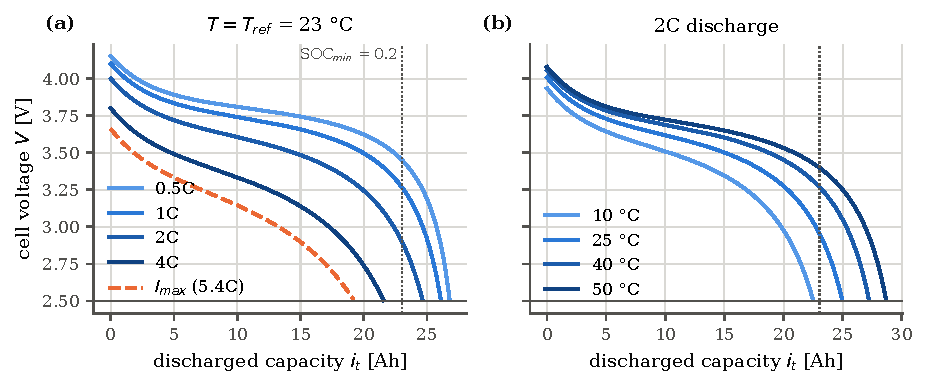
\includegraphics[width=\textwidth]{figures/fig_cell_discharge.pdf}
\caption{Constant-current discharge of the rescaled cell of \code{hybrid_config('II')}
(Eq.~\eqref{eq:shepherd} at constant $T$). (a)~C-rates referred to $Q_0=28.78$~Ah, at
$T_{ref}$; the dashed curve is the current limit $I_{max}=155.2$~A. (b)~2C at four
temperatures. Curves stop at $V_{min}=2.5$~V (solid grey line) or at $i_t\to Q_0$. The dotted
line marks $\mathrm{SOC}_{min}=0.2$. Script: \code{fig_cell.py}.}
\label{fig:discharge}
\end{figure}

\begin{figure}[t]
\centering
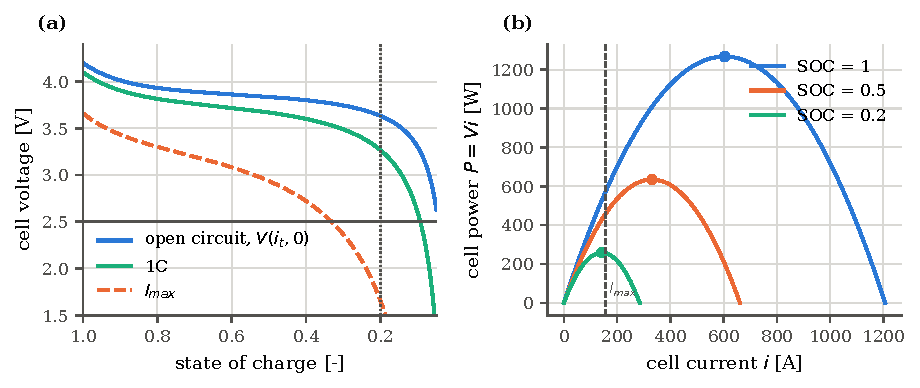
\includegraphics[width=\textwidth]{figures/fig_cell_power.pdf}
\caption{(a)~Open-circuit and loaded cell voltage versus SOC at $T_{ref}$. (b)~Cell power
$P=V\,i$ versus current at three SOC values, the quadratic of Eq.~\eqref{eq:quadratic}. Dots
mark the apex $b^2/(4|a|)$; the dashed line is $I_{max}$. Script: \code{fig_cell.py}.}
\label{fig:power}
\end{figure}

Figure~\ref{fig:discharge}(a) shows how the C-rate shifts the curve. At $T_{ref}$ the voltage
at $\mathrm{SOC}_{min}$ is 3.45~V at 0.5C, 3.27~V at 1C and 2.90~V at 2C. At 4C the cell
reaches $V_{min}$ after 21.55~Ah, before $\mathrm{SOC}_{min}$ (23.03~Ah). At $I_{max}$ it
reaches $V_{min}$ after 19.20~Ah ($\mathrm{SOC}=0.33$). A pack that flies close to its current
limit is therefore voltage limited before it is energy limited. Figure~\ref{fig:discharge}(b)
shows the temperature effect, which acts through both $Q(T)$ and $R(T)$. At 10\degC\ the
capacity is $Q=27.24$~Ah and the resistance is 1.55 times its reference value, so the 2C
discharge reaches $V_{min}$ after 22.49~Ah, just before $\mathrm{SOC}_{min}$ (23.03~Ah). At 40
and 50\degC\ $Q(T)$ exceeds $Q_0$ and the resistance falls, so the SOC limit is reached first.

\subsection{Limits and error codes}
\label{sec:limits}

The cell model validates its own state through property setters. A violation raises
\code{BatteryError} with a code (Table~\ref{tab:errors}). The mission catches the exception and
reports the pack size as infeasible. Temperature is \emph{not} limited by an error: the
ceiling acts through the thermostat of Section~\ref{sec:thermal}, and only a negative
temperature raises.

\begin{table}[h]
\centering\small
\caption{Checks of the Class-II battery (\code{Battery.py}).}
\label{tab:errors}
\begin{tabular}{@{}p{3.6cm}p{3.6cm}p{7.6cm}@{}}
\toprule
Code & Raised by & Condition\\
\midrule
\code{SOC_OUTSIDE_LIMITS} & setter \code{it}, property \code{SOC} & $\mathrm{SOC}<\mathrm{SOC}_{min}$ or $\mathrm{SOC}>1$, Eq.~\eqref{eq:soc}\\
\code{VOLTAGE_OUTSIDE_LIMITS} & property \code{cell_Vout} & $V<V_{min}$ (no upper check)\\
\code{CURR_OUTSIDE_LIMITS} & property \code{cell_i} & $i>I_{max}$\\
\code{BATT_UNDERPOWERED} & setter \code{i} & negative discriminant in Eq.~\eqref{eq:quadratic}\\
\code{NEG_BATT_TEMP} & setter \code{T} & $T<0$~K\\
\code{PACK_HEAVIER_THAN_AIRCRAFT} & \code{find_parallel_cells} & the pack as heavy as the aircraft is infeasible (Section~\ref{sec:psearch})\\
\texttt{REQUIRES\_CLASS\_II}, \code{NO_CHARGE_C_RATE} & \code{thermal_degradation_analysis} & wrong class, or no positive charge C-rate\\
(no code) & \code{SOC_min}, \code{T} getters & minimum SOC or temperature unset, $\mathrm{SOC}_{min}\notin[0,1]$\\
\bottomrule
\end{tabular}
\end{table}

The setter of \code{cell_max_current} also checks that $V(0,I_{max})\ge V_{min}$, and raises a
\texttt{ValueError} otherwise. This protects the rescaling of Section~\ref{sec:rescale} from a
current limit that the cell cannot carry.

\subsection{Lumped thermal model}
\label{sec:thermal}

Each cell is a single thermal node of capacity $C_{th}$ [J/K]. \code{Battery.heatLoss}
returns the temperature derivative and the heat generated per cell:
\begin{equation}
\dot q = (V_{oc}-V)\,i - \frac{\partial E}{\partial T}\,i\,T,\qquad
\frac{dT}{dt} = \frac{\dot q}{C_{th}} + \frac{T_a - T}{R_{th}\,C_{th}},\qquad
R_{th} = \frac{1}{h\,A_s} + R_{i,th}.
\label{eq:thermal}
\end{equation}
This is the Bernardi heat for a discharge current $i>0$. The first term of $\dot q$ is the
irreversible heat of the overpotentials; the second is the reversible (entropic) heat, which with
$\partial E/\partial T>0$ is absorbed in discharge. At low current $\dot q$ can therefore be
negative. The model constants are assumptions of the code:
\begin{itemize}
\item $C_{th}=1000\,m_c$ [J/K], a specific heat of 1000~J/(kg\,K);
\item $R_{i,th}=3.3\,(r_c/0.022)^2$ [K/W], the conduction resistance inside the cell. The
  structure of an internal resistance in series with the convection to the air follows Forgez
  et al.\ (J.~Power Sources 195 (2010) 2961--2968), as described in the MSc thesis of
  J.~Delille that introduced the thermal model (\code{research/Alan_FC/Tesi_Joao/Thesis_Joao.pdf},
  Sections 2.1.3 and 2.3.3). The thesis attributes the thermal parameters to Saw et al.\
  (J.~Power Sources 249 (2014) 231--238) and to Forgez et al. Neither the thesis nor any other
  file of the repository states the value 3.3~K/W or the reference radius 0.022~m, so the
  value is uncited;
\item $A_s=2\pi r_c h_c$, the lateral surface of the cylinder;
\item the cooling flow $\dot m = \max(10^{-4}\,\dot q,\,0)$ and the convective coefficient
\begin{equation}
h = \max\left[30\left(\frac{\dot m/(A_m\,\rho)}{5}\right)^{0.8},\;2\right]\ \mathrm{W/(m^2K)},
\end{equation}
where $A_m=(2r_c)^2-\pi r_c^2$ is the free cross-section around one cell and $\rho$ the
ambient density. The code cites \url{http://dx.doi.org/10.1016/j.jpowsour.2013.10.052} for
this law. The ambient temperature is clipped to at least 273.15~K.
\end{itemize}

A thermostat is layered on top of Eq.~\eqref{eq:thermal}. Inside \code{heatLoss}, $h=0$
(adiabatic pack) while the battery discharges ($\varphi>0$) and $T$ is below the ceiling
$T_{lim}$ (\texttt{'Max operative temperature'}). The mission right-hand side then clamps the
derivative (\code{Mission.HybridConfigurationClassII.model}, and the same logic in the other
Class-II paths):
\begin{equation}
\frac{dT}{dt} \leftarrow
\begin{cases}
\max(dT/dt,\,0) & \varphi>0,\ T<T_{lim},\\
0 & \varphi>0,\ T\ge T_{lim},\\
\min(dT/dt,\,0) & \varphi=0.
\end{cases}
\label{eq:thermostat}
\end{equation}
In words: the pack heats adiabatically until the ceiling, is held there by a cooling system
that removes exactly the generated heat, and relaxes toward the ambient air when the battery is
idle. At $\varphi=0$ the current is zero, $\dot q=0$, and only the natural-convection floor
$h=2$~W/(m$^2$K) acts.

For the rescaled cell at 2C and half charge the irreversible heat is 19.22~W and the entropic
term absorbs 0.84~W, so $\dot q=18.38$~W.

%======================================================================
\section{Class II sizing inside the mission}
\label{sec:classII-sizing}
%======================================================================

The Class-II pack has no closed-form mass. The mission searches for the smallest number of
parallel cells $P$ that flies the whole mission within the limits of Table~\ref{tab:errors}, and
the weight loop uses the resulting \code{pack_weight}.

\subsection{Mission states}

\code{Mission.HybridConfigurationClassII} integrates five states,
$\mathbf{y}=[E_f,\,E_b,\,\beta,\,i_t^{pack},\,T]$, with $i_t^{pack}$ in A\,s:
\begin{equation}
\frac{d\mathbf{y}}{dt} = \left[P_p\Pi_0,\; i\,V_{pack},\; -\frac{P_p\Pi_0}{e_f W_{TO}},\; i,\;
\frac{dT}{dt}\right].
\label{eq:classII-ode}
\end{equation}
At each evaluation the right-hand side sets $T$, then $i_t=i_t^{pack}/3600$ (checking the
SOC), then the pack current from Eq.~\eqref{eq:quadratic} with $P_{el}=P_p\Pi_5$ (checking the
discriminant and the current), and evaluates $V_{pack}$ (checking the voltage). It computes
$dT/dt$ from Eqs.~\eqref{eq:thermal}--\eqref{eq:thermostat} with the ISA ambient temperature
and density. The battery energy $E_b=\int iV_{pack}\,dt$ is the terminal energy. Each segment is
integrated with BDF at \code{rtol=1e-6}. A \code{BatteryError} anywhere in a segment, including
in a trial state of the implicit solver, aborts the evaluation.

After each segment the code re-evaluates the right-hand side at every output point to store
\code{Mission.plottingVars} $=[t,\mathrm{SOC},V_{oc}^{pack},V^{pack},i^{pack},T,T_a,h,\dot m]$.
If a stored point violates a limit, the code prints ``WARNING: evaluate\_P\_number integration
rtol may be too loose'' and continues; the design is not affected. The fuel-cell variant
\code{Mission.FuelCellBatteryConfigurationClassII} uses the same five states, with
the battery delivering $\varphi P_p/\eta_{el}$ at its terminals. It does not fill
\code{plottingVars}.

\subsection{Ground legs and the take-off check}
\label{sec:pack-ground}

Before the climb, \code{Mission._pack_before_climb} flies the pack from full charge
at the initial temperature through three steps. First, taxi-out at constant terminal power.
Second, an instantaneous check that the pack can deliver the worst-case take-off/OEI battery
power $P_{bat,TO}$ at the state after taxi-out (current and voltage checks). Third, the
take-off run. \code{Mission._pack_through_ground_legs} integrates each leg with the
in-flight thermal logic at the take-off altitude; taxi is evaluated at zero airspeed and the
take-off run at the take-off speed. After landing, the same function flies taxi-in from the
final pack state. A leg without battery power is skipped. Any failure makes the $P$
infeasible. Section~\ref{sec:ground} gives the power of these legs.

\subsection{The P-number search}
\label{sec:psearch}

For a given take-off mass $W_{TO}$, the function \code{find_parallel_cells} of
\code{Battery.py} finds the smallest feasible integer $P$. Both Class-II mission
methods call it through their nested \code{find_P_nr}. The nested function
\code{evaluate_mission_given_P(P)} calls \code{Configure(P)}, flies the ground legs and the
profile, and returns \texttt{(True, None)} or \texttt{(False, code)}; for $P=0$ it returns
\texttt{(False, None)} without flying. The search assumes that feasibility is monotone in $P$.
Its doubling step does not go beyond the pack that is as heavy as the aircraft:
\begin{equation}
P_{lim} = \left\lfloor \frac{W_{TO}}{S\,m_c} \right\rfloor,
\end{equation}
where $m_c$ is the cell mass. The steps are:
\begin{enumerate}
\item \emph{Initial bracket.} On the first weight-loop call, $P_{max}=128$ (hard-coded) and
  $P_{min}=\lfloor P_{max}/2\rfloor$. On later calls, $P_{max}=\lceil P^{*}\,W_{TO}/W_{TO,last}\rceil$
  and $P_{min}=P_{max}-1$, where $P^*$ is the previous optimum.
\item \emph{Lower bound.} While $P_{min}$ is feasible, set $P_{max}\leftarrow P_{min}$ and halve
  $P_{min}$.
\item \emph{Upper bound.} If no feasible $P_{max}$ is known yet, double $P_{max}$ until it is
  feasible, moving the old value to $P_{min}$. The doubling stops at $P_{lim}$. If $P_{lim}$, or
  a larger first guess, is infeasible, the search raises a \code{BatteryError} with code
  \code{PACK_HEAVIER_THAN_AIRCRAFT}.
\item \emph{Bisection.} Bisect between the infeasible $P_{min}$ and the feasible $P_{max}$ until
  a feasible $P$ with $P-P_{min}=1$ is found.
\end{enumerate}
The optimum is kept in \code{Mission.optimal_n}, and the list of evaluated $P$ of each call is
appended to \code{Mission.Past_P_n}. The last flight of a search is always the returned $P$,
so the mission histories and \code{Mission.battery_end_state} belong to the sized pack. When
\code{Mission.size_battery_pack} is \texttt{False}, the pack is not resized: the mission flies
the configured $P$ and returns \texttt{(0, code)} on a failure. The off-design tools use this
mode.

The error of the upper bound leaves the mission and reaches the weight loop. In
\code{Weight.Hybrid}, \code{Weight._solve_wto} first runs Brent's method on the whole bracket.
When that fails, it scans the bracket in steps of 10\,000~kg, treats a take-off mass at which
the search raises as having no residual, and runs Brent's method on the first step that
brackets a root. When no step brackets a root, it raises the original error.
\code{Weight.FuelCellBattery} lets the \code{BatteryError} through unchanged. Whenever a pack
not heavier than the aircraft is feasible, the bounded search returns the same $P$ as an
unbounded one, so the bound does not change a feasible design. In the baseline search below,
the heaviest evaluated pack is 8.6~\% of the take-off mass at which it was evaluated.

Figure~\ref{fig:psearch} shows the search on \code{hybrid_config('II')}. The weight loop
(\code{Weight._solve_wto} with Brent's method on $[10\,000, 60\,000]$~kg) calls the mission
seven times. The search evaluates the mission 41 times in total, and the design took
between 17 and 26~s in the runs made for this manual, depending on the machine load. The first two calls are the bracket ends of Brent's
method, so their $P$ (51 and 304) are far from the result. The later calls start from the scaled
previous optimum. The fourth, sixth and seventh need three evaluations. In the third and the
fifth the scaled guess (105, then 110) is already feasible, so the halving restarts the bracket
at half that value and the bisection needs eight evaluations. Flying the converged design with
$P=109$ or $P=108$ fails with \texttt{SOC\_OUTSIDE\_LIMITS}, which confirms that $P=110$ is the
smallest feasible pack.

\begin{figure}[t]
\centering
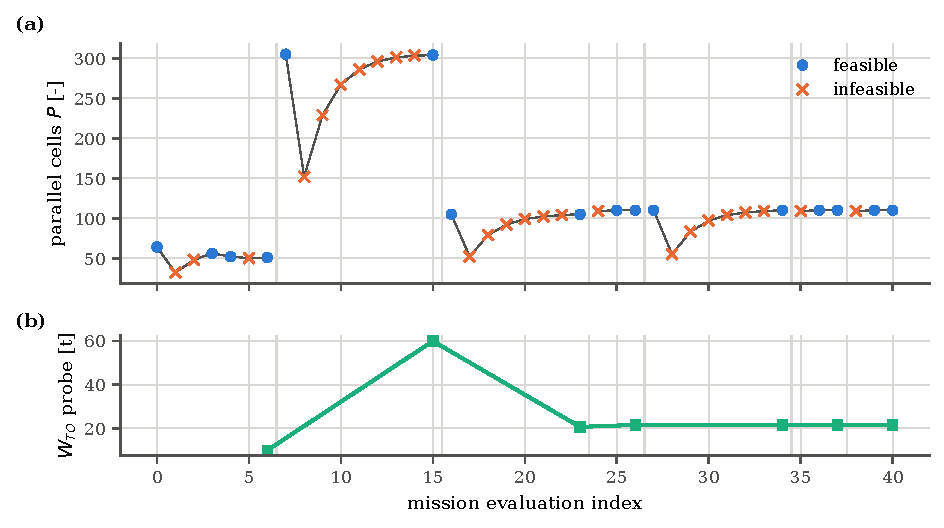
\includegraphics[width=\textwidth]{figures/fig_pnumber_search.pdf}
\caption{P-number search on \code{hybrid_config('II')}. (a)~Every evaluated $P$, in order;
vertical lines separate the weight-loop calls. Feasibility is inferred from monotonicity: a
$P$ is marked feasible if it is not below the optimum of its call. (b)~Take-off mass at which
each call was made. Data: \code{Mission.Past_P_n}; script: \code{fig_class_ii_mission.py}.}
\label{fig:psearch}
\end{figure}

\subsection{The sized baseline}

The converged design has $W_{TO}=21\,630$~kg and a pack of $S\times P=190\times110=20\,900$
cells, 1483.9~kg. The pack holds a nominal 2226~kWh and can deliver 11.97~MW, and the mission
draws 1842~kWh at its terminals. The Class-I design with the same specific energy and power
gives 1542.6~kg and $W_{TO}=21\,742$~kg.

Figure~\ref{fig:mission} shows the time histories. The battery works only in cruise, from
27.3 to 159.5~min, where $\varphi$ ramps to 0.5. The SOC falls from 1 to 0.204 and stays
there. The peak cell current is 16.4~A, about 0.57C and a tenth of $I_{max}$. The lowest
terminal cell voltage is 3.67~V. Therefore this pack is limited by the SOC, as the Class-I
energy candidate is. During the climb the idle pack cools from 25\degC\ to 20.5\degC, because
$\varphi=0$ there and Eq.~\eqref{eq:thermostat} lets it relax toward the colder ambient air. In
cruise it heats adiabatically and reaches the 50\degC\ ceiling at 142.3~min. From then until
the end of cruise the thermostat holds it there, and in the
descent and diversion it cools toward ambient, reaching 25.9\degC\ at the end of the mission.

\begin{figure}[p]
\centering
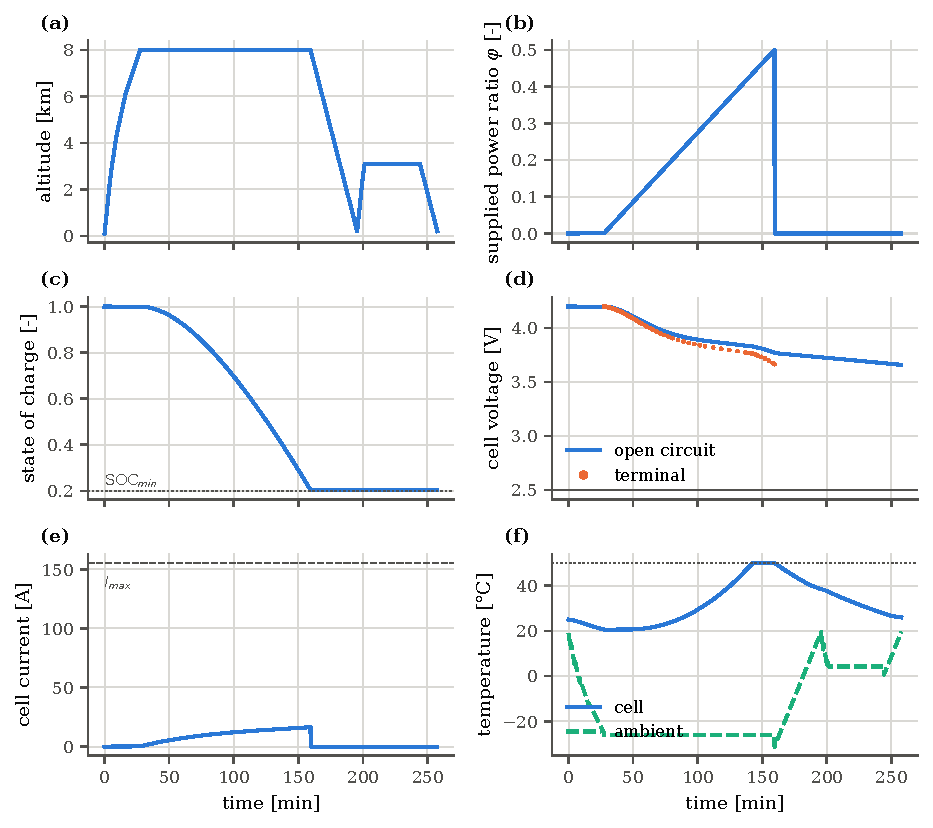
\includegraphics[width=\textwidth]{figures/fig_mission_class_ii.pdf}
\caption{Class-II pack along the mission of \code{hybrid_config('II')} (data:
\code{Mission.plottingVars} of the last evaluation, so ground legs are not shown). (a)~altitude;
(b)~$\varphi(t)$; (c)~SOC; (d)~cell open-circuit and terminal voltage, the latter only where
$\varphi>0$; (e)~cell current and $I_{max}$; (f)~cell and ambient temperature, with the
50\degC\ ceiling dotted. Script: \code{fig_class_ii_mission.py}.}
\label{fig:mission}
\end{figure}

\subsection{Battery cooling mass}
\label{sec:hex}

With the thermostat of Eq.~\eqref{eq:thermostat}, heat leaves the pack only while it is held
at the ceiling. After the mission is sized, \code{HybridConfigurationClassII} (and its fuel-cell
counterpart) scans the integration points with $T\ge T_{lim}-0.5$~K, recomputes the cell heat
$\dot q$ and stores the peak pack value $\dot Q_{bat}=\max(SP\,\dot q)$ as
\code{Mission.Max_Bat_Thermal_Pwr}. The weight loop adds a cooling mass
\begin{equation}
W_{HEX,bat} = \frac{\dot Q_{bat}}{p_{HEX,bat}},
\label{eq:hex}
\end{equation}
where $p_{HEX,bat}$ is \texttt{'HEX Specific Power Battery'} (default 1500~W/kg). The term is
part of \code{Weight.WHeat_Exchanger} in \code{Weight.Hybrid}. In \code{Weight.FuelCellBattery}
it is added to the fuel-cell thermal-management mass described in the Thermal Management
manual. The Class-I battery has no thermal model and carries no cooling mass. If the pack never
reaches the ceiling, $\dot Q_{bat}=0$.

Figure~\ref{fig:heat} shows the pack heat of the baseline. The heat generated grows with the
current through the cruise. The cooling system rejects it from 142.3~min, and the peak is
30.1~kW at the end of cruise. Equation~\eqref{eq:hex} gives 20.0~kg. The heat stored in the
thermal mass before the ceiling is not counted, and neither is the cooling during idle phases,
which is passive.

\begin{figure}[t]
\centering
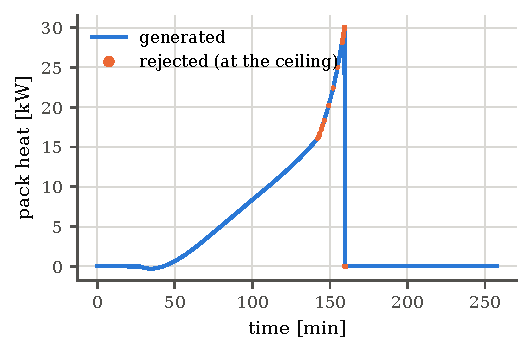
\includegraphics[width=0.62\textwidth]{figures/fig_pack_heat.pdf}
\caption{Pack heat generation along the mission of \code{hybrid_config('II')}, and the points
at the temperature ceiling, from which \code{Max_Bat_Thermal_Pwr} is taken. Script:
\code{fig_class_ii_mission.py}.}
\label{fig:heat}
\end{figure}

%======================================================================
\section{Powertrain coupling}
\label{sec:powertrain}
%======================================================================

The battery is coupled to the rest of the aircraft through the power ratios of the powertrain
graph, the sizing of the electric drive, and the energy accounting downstream of the design.

\subsection{Hybrid power ratios}

\code{Powertrain.Hybrid(phi, alt, vel, pwr)} assembles a linear system of normalized
powers with the primitives of \code{Systems/Powertrain/graph.py}. A \emph{converter} imposes
$P_{out}=\eta P_{in}$, a \emph{combiner} $P_{out}=\eta\sum P_{in}$, the \emph{split} imposes
Eq.~\eqref{eq:phi-hybrid}, and a \emph{sink} sets $P_p=1$. For the parallel architecture
(\code{parallel_hybrid_graph}) the unknowns are
$[P_f, P_{gt}, P_{gb}, P_{s1}, P_{e1}, P_{bat}, P_{p1}]$ and the equations are
\begin{equation}
P_{gt}=\eta_{gt}P_f,\quad P_{s1}=\eta_{gb}(P_{gt}+P_{gb}),\quad P_{e1}=\eta_{pm}P_{bat},\quad
P_{gb}=\eta_{em}P_{e1},\quad P_{p1}=\eta_{p}P_{s1},
\end{equation}
plus the split and $P_{p1}=1$. The serial architecture (\code{serial_hybrid_graph})
places the battery on the electrical bus after the generator:
$P_{s1}=\eta_{em1}P_{gt}$, $P_{e1}=\eta_{pm}(P_{s1}+P_{bat})$, and the motor, gearbox and
propeller in series. The solution vector is returned in absolute value. Its entry 5 is
$\Pi_5=P_{bat}/P_p$, the battery terminal power per unit propulsive power used in
Eqs.~\eqref{eq:classI-ode} and \eqref{eq:classII-ode}. Entry 0 is the fuel and entry 1 the
gas-turbine shaft power. Entry 2 is the electric-motor shaft power and entry 4 the electric power
into the motor; the serial sizing below uses them. The efficiencies come from \code{Powertrain.eta}, which supports
operating-point dependent models. Each model is evaluated at the power through its own
component (\code{Powertrain._solve_at_component_powers}): the motor at its shaft output, the
PMAD at its input, the serial generator at its electrical output. With constant efficiencies
the first solve is returned. The serial generator is the \texttt{'generator'} entry
(\code{EtaEM1}) and the serial motor the \texttt{'electric\_motor'} entry (\code{EtaEM2}).

\subsection{Electric motor and PMAD}
\label{sec:motor}

\code{Powertrain.WeightPowertrain} sizes the electric drive of a \texttt{'Hybrid'}.
In the parallel architecture the motor and the PMAD carry only the battery power, so both are
sized on the peak battery power:
\begin{equation}
P_{bat,peak} = \max(P_{bat,max},\,P_{bat,TO}),\qquad
W_{motor} = \frac{P_{bat,peak}}{p_{em}},\qquad W_{PMAD} = \frac{P_{bat,peak}}{p_{PMAD}},
\end{equation}
with $p_{em}$ the second entry of \texttt{'Specific Power Powertrain'} and $p_{PMAD}$ the
\texttt{'Specific Power PMAD'} (default 10\,000~W/kg, \code{pmad_specific_power}). On the
Class-II baseline the motor weighs 251.4~kg and the PMAD 125.7~kg for $P_{bat,peak}=1.257$~MW.

In the serial architecture the motor carries the whole shaft power to the propeller, the
generator the whole turbine power and the PMAD the whole bus power. The mission therefore also
tracks the motor shaft power $P_{mot}=P_p\Pi_2$ and the bus power $P_{bus}=P_p\Pi_4$, as peaks over
the profile (\code{Max_PMotor}, \code{Max_PBus}) and at the take-off/OEI point
(\code{TO_PMotor}, \code{TO_PBus}). This holds in \code{HybridConfigurationClassI},
\code{HybridConfigurationClassII} and the range extender. The sizing is
\begin{equation}
W_{motor+gen} = \frac{\max(P_{mot,max},P_{mot,TO})}{p_{em}} + \frac{P_{eng}}{p_{gen}},\qquad
W_{PMAD} = \frac{\max(P_{bus,max},P_{bus,TO})}{p_{PMAD}},
\end{equation}
where $P_{eng}$ is the engine rating and $p_{gen}$ the \texttt{'Specific Power Generator'}
(\code{specific_power_generator}). Its default is the motor value $p_{em}$, and
\code{examples/common.py} writes it explicitly at 5000~W/kg, equal to $p_{em}$. The code stores
the generator mass as \code{Powertrain.WGenerator} and the sum as \code{Powertrain.WMotor}. On
\code{hybrid_config('I', 'Serial')} the motor peak is 4.95~MW and the engine rating 5.92~MW, so
the motor and generator weigh 2174.1~kg and the PMAD 515.6~kg (bus peak 5.16~MW). The battery,
1373~kW peak before this sizing, is not the driver; the take-off mass is 31\,034~kg against
21\,742~kg for the parallel Class-I design. The Class-II nominal-power check
\code{Powertrain.report_class_ii_sizing} compares \code{Max_PBat} with \texttt{'EM Design
Power'} when the latter is given.

\subsection{Serial range extender}
\label{sec:re}

\code{Mission.SerialRangeExtenderConfiguration} runs the turbine at its rated
shaft power, lapsed with altitude by the ISA pressure ratio
(\code{_range_extender_gt_power}). At each instant \code{_range_extender_flows} computes the
battery terminal power
\begin{equation}
P_{bat} = \frac{P_p}{\eta_p\,\eta_{gb}\,\eta_{em2}\,\eta_{pm}} - \eta_{em1}P_{gt},
\end{equation}
positive when discharging and negative when the turbine surplus recharges the pack. The state
$E_{rem}$ integrates $P_{bat}$ in discharge and $\eta_{ch}P_{bat}$ in charge, with
$\eta_{ch}$ = \texttt{'Battery Charge Efficiency'} (default 1.0). The battery energy returned
to the weight loop is the \emph{swing}
\begin{equation}
E_{swing} = \max_t E_{rem}(t) - \min_t E_{rem}(t),
\end{equation}
taken over the energy levels after taxi-out, after the take-off run, along the flight and
after taxi-in. The take-off run is flown with the turbine at full throttle and the battery
covering the rest, ignoring $\varphi_{TO}$. Equation~\eqref{eq:classI-mass} then sizes a
Class-I pack on $E_{swing}$, and \code{_add_ground_energy} does not add the ground energy again.
With \code{hybrid_config('I', 'Serial')}, a rated power of 3.0~MW (constant turbine efficiency)
and $\eta_{ch}=0.96$, the swing is 3713~kWh and the pack 3094~kg, energy limited, for a take-off
mass of 29\,475~kg. The ground legs draw 75.8~MJ, all in the take-off run, where the battery
delivers 1.80~MW. The motor and generator weigh 1541.1~kg on a motor peak of 4.71~MW plus the
3.0~MW rating. The range extender has no Class-II path and no
$\varphi$ split, and \code{examples/30_off_design_mission.py:fly_off_design} rejects it.

\subsection{Fuel cell and battery}

In \texttt{'FuelCellBattery'} the split is applied directly to the propulsive power: the fuel
cell supplies $(1-\varphi)P_p$ through its own efficiency (\code{FuelCell.ComputePRatio}, see
the Fuel Cell manual) and the battery $\varphi P_p$ through the chain
$\eta_{el}=\eta_{EM}\eta_{PM}\eta_{GB}\eta_{prop}$, which includes the propeller as the fuel-cell
branch does. \code{FuelCell.drive_efficiencies} returns $\eta_{EM}$ and $\eta_{prop}$: constants
by default, the powertrain \texttt{'propeller'} model when the Hamilton propeller is attached,
and the d-q motor model when \texttt{'Eta Electric Motor Model'} is \texttt{'Smart'}. The battery
energy and powers handed to the weight loop are terminal quantities
(\code{Mission._fc_battery_terminal_power}). Only the hydrogen burn changes the mass. The battery
energy of the Class-I path is a post-processed integral; the Class-II path integrates it as a
state. The ground segments carry battery power at $\varphi_{TO}$ and $\varphi_{taxi}$
(Section~\ref{sec:ground}).

The stack is sized on $\max$(mission peak, take-off, OEI) of its own share $(1-\varphi)P_p$.
The battery feeds the same PMAD and motor as the fuel cell, so \code{FuelCell._size_stack}
sizes both on \code{Mission.Max_PDrive}, the peak propulsive power through the drive at one
instant (fuel-cell and battery shares together, over the mission, the take-off/OEI point and
the ground legs). It is never below the fuel-cell share, so a design with $\varphi=0$ is
identical to the \texttt{'Hydrogen'} one. A take-off battery therefore shrinks the stack only
when the take-off sets it, and the motor and PMAD still carry the full take-off power (see the
Fuel Cell manual and example \code{23_fuelcell_battery_hybrid.py}).
\code{Powertrain.PowerRatioFuelCellBattery} and
\code{graph.fuelcell_battery_graph} express the same architecture as a graph but are not used by
the mission.

\subsection{Downstream energy accounting}

\code{Weight.TotalEnergies} $=[E_f, E_b]$ feeds two post-design modules. The well-to-wake
module (\code{WellToWake.EvaluateSource}) divides $E_b$ by
$\eta_{CH}\eta_{GR}$ (\texttt{'Eta Charge'}, \texttt{'Eta Grid'}, both default 1.0) to get the
source energy, and reports the electric share $\Psi$. The climate module
(\code{ClimateImpact._grid_battery_co2}) multiplies the same source energy by
\texttt{'Grid\_CO2'} [kg~CO$_2$/MJ]. In both cases $E_b$ is the terminal energy drawn from the
pack; the charging efficiency of the cell itself is not modelled.

%======================================================================
\section{Ground segments}
\label{sec:ground}
%======================================================================

Taxi-out, the take-off run and taxi-in are not part of the flown profile.
\code{Mission._ground_segments} computes their energy before the mission is flown,
and the battery takes a share of it.

The reference power is the take-off-field propulsive power $P_{TO}$
(\code{Mission._takeoff_power}). The take-off run lasts $t_{TO}$ (\texttt{takeoff\_time},
default 0.7~min) at $f_{TO}P_{TO}$ (\texttt{takeoff\_power\_fraction}, default 1.0). Taxi-out
and taxi-in last $t_{out}$ and $t_{in}$ (default 13~min each) at $f_{taxi}P_{TO}$
(\texttt{taxi\_power\_fraction}, default 0.07). The defaults are the ICAO LTO reference values
cited in the code. \code{Mission._ground_power_split} splits each power through the
configuration's own powertrain at the take-off condition. The battery takes $\varphi_{TO}$ of
the take-off power and $\varphi_{taxi}$ of the taxi power, with the meaning of $\varphi$ of
Section~\ref{sec:phi}. It returns the fuel chemical power $P_f$, the battery terminal power
$P_{el}$ and the battery sizing power, which is the terminal power in every configuration (the
range extender counts only discharge). The take-off condition is the take-off altitude and the
true airspeed from \code{Mission._ground_condition}; the take-off/OEI power ratios of the mission
methods (\code{TO_PBat}, \code{TO_PP}) are evaluated at the same condition. Then
\begin{align}
E_{f,ground} &= t_{TO}P_{f,TO} + (t_{out}+t_{in})P_{f,taxi}, &
E_{b,ground} &= t_{TO}P_{el,TO} + (t_{out}+t_{in})P_{el,taxi},\\
\beta_0 &= 1 - \frac{t_{TO}P_{f,TO}+t_{out}P_{f,taxi}}{e_f\,W_{TO}}, &
P_{bat,max} &\leftarrow \max(P_{bat,max},\,P_{bat,taxi},\,P_{bat,takeoff}).
\end{align}
\code{Mission._add_ground_energy} adds $E_{f,ground}$ and $E_{b,ground}$ (stored as
\code{E_ground} and \code{EBat_ground}) to the energies returned by the mission method, except
for the range extender (Section~\ref{sec:re}). \code{Mission.EvaluateMission} folds
\code{Taxi_PBat} and \code{Takeoff_PBat} into \code{Max_PBat}. A non-zero
\texttt{'Taxi Supplied Power Ratio'} on a configuration without a battery raises a
\texttt{ValueError} in \code{Mission.SetInput}. The Class-II pack flies the same legs
(Section~\ref{sec:pack-ground}).

Figure~\ref{fig:taxi} shows the effect of $\varphi_{taxi}$ on \code{hybrid_config('I')}
($\varphi_{TO}=0$). With $\varphi_{taxi}=1$ the battery supplies 370.1~MJ on the ground and
the ground fuel falls from 2240~MJ to 628~MJ, the take-off run alone. The battery grows by
100.5~kg, the fuel falls by 21.4~kg, and the take-off mass grows by 190.4~kg. The curve is not
linear in $\varphi_{taxi}$ because of Eq.~\eqref{eq:phi-hybrid}: at $\varphi_{taxi}=0.25$ the
battery already supplies 219.5~MJ, 59~\% of the all-electric value. On \code{hybrid_config('II')}
the electric taxi raises the pack from $P=110$ to $P=117$ (1578.3~kg). The climb then starts
with 64.5~Ah drawn from the pack, an SOC of 0.981, and the cell still at 25.0\degC: at the low
taxi current the thermostat keeps the adiabatic pack from cooling, and the take-off run is
flown with $\varphi_{TO}=0$.

\begin{figure}[t]
\centering
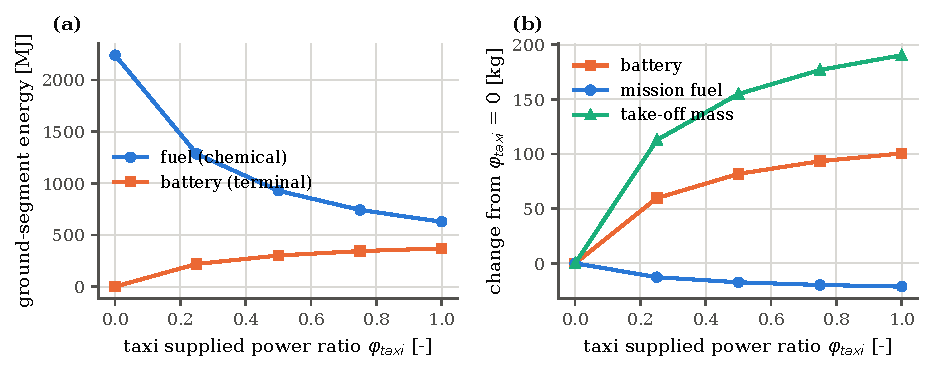
\includegraphics[width=\textwidth]{figures/fig_taxi_phi.pdf}
\caption{Taxi supplied power ratio on \code{hybrid_config('I')}. (a)~Ground-segment energy:
fuel chemical and battery terminal. (b)~Change of battery, mission fuel and take-off mass from
the fuel-only taxi. Script: \code{fig_sizing_studies.py}.}
\label{fig:taxi}
\end{figure}

%======================================================================
\section{State of health and ageing}
\label{sec:soh}
%======================================================================

PhlyGreen represents battery ageing in two separate ways. A prescribed state of health enters
the design and the off-design flights. A post-design analysis estimates the ground fast-charge
load and the cycle life. Mission-driven ageing estimators are not implemented.

\subsection{State of health}

\code{Battery.set_state_of_health(capacity_fraction, resistance_factor)} sets the
capacity fraction $c=C/C_{BOL}\in(0,1]$ and the resistance factor $r=R/R_{BOL}>0$ relative to
the beginning of life (BOL). The BOL values are stored in \code{Battery._bol} by \code{SetInput},
so the call is idempotent and \code{set_state_of_health()} restores BOL. The scaling is:
\begin{itemize}
\item Class II: $Q_0\leftarrow cQ_0$, $E_{nom}\leftarrow cE_{nom}$,
  $\partial Q/\partial T\leftarrow c\,\partial Q/\partial T$, $B\leftarrow B/c$, $R\leftarrow rR$,
  $K\leftarrow rK$. The Arrhenius constants, $I_{max}$, $S$ and the cell mass do not change.
  The cell model then enforces the limits of the aged cell.
\item Class I (\texttt{CellInput}): $E_{bat}\leftarrow cE_{bat}$ and $p_b\leftarrow p_b/r$.
  Dividing the specific power by $r$ is a first-order approximation stated in the docstring: the
  deliverable power is inversely proportional to the internal resistance.
\item Class I of \texttt{'FuelCellBattery'}: the factors are read in
  \code{Weight.FuelCellBattery}, Eq.~\eqref{eq:fcb-mass}.
\end{itemize}
The inputs are \code{EnergyConfig.battery_capacity_fraction} and
\code{EnergyConfig.battery_resistance_factor} (\texttt{'Battery Capacity Fraction'},
\texttt{'Battery Resistance Factor'}). \code{Aircraft.ReadInput} applies them after the battery
\code{SetInput}, for every battery model. Set before the design, they size the pack at end of
life (EOL). Applied to a copy of a sized aircraft, they fly an aged pack.

\subsection{End-of-life sizing}

Figure~\ref{fig:soh-sizing} shows EOL sizing. On \code{hybrid_config('I')}, $c=0.8$ raises the
battery from 1542.6 to 2062.4~kg, a factor 1.337, and $W_{TO}$ from 21\,742 to 23\,254~kg. The
factor exceeds $1/c=1.25$ because the heavier aircraft needs more energy (1980 against
1851~kWh). The Class-II pack follows closely: $c=0.9$ and 0.8 give $P=125$ and $P=146$, that is
1686.2 and 1969.5~kg. The resistance factor acts differently. On the energy-limited Class-II
pack, $r=2$ adds four strings ($P=114$, +3.6~\%) because the larger drop lowers the voltage and
draws more charge for the same terminal energy. It also raises the heat at the ceiling, and the
cooling mass of Eq.~\eqref{eq:hex} grows from 20.0~kg to 33.7~kg at $r=1.5$ and 49.2~kg at
$r=2$. On the power-limited take-off
battery ($\varphi_{TO}=0.3$, cruise $\varphi=0$) the Class-I pack grows from 258.3~kg to 396.1~kg
at $r=1.5$ and 540.3~kg at $r=2$.

\begin{figure}[t]
\centering
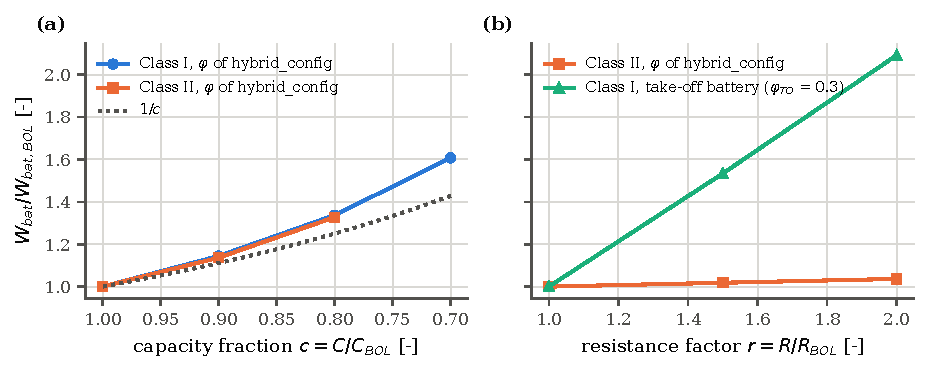
\includegraphics[width=\textwidth]{figures/fig_soh_sizing.pdf}
\caption{End-of-life sizing: battery mass relative to the BOL design. (a)~Capacity fraction on
\code{hybrid_config} (Class I and Class II); dotted: $1/c$. (b)~Resistance factor on the
Class-II \code{hybrid_config} (energy limited) and on a Class-I take-off battery
($\varphi_{TO}=0.3$, power limited). Script: \code{fig_sizing_studies.py}.}
\label{fig:soh-sizing}
\end{figure}

\subsection{Aged flight of a sized pack}

\code{examples/30_off_design_mission.py:fly_off_design(sized, range_nm, ...,
state_of_health=...)} flies a deep copy of a sized aircraft. The dictionary
\texttt{state\_of\_health} uses the \texttt{EnergyConfig} keys. Off-design, the take-off mass is
closed by a fixed-point iteration on the fuel. A Class-I pack is checked against its usable
energy $W_{bat}E_{bat}(1-\mathrm{SOC}_{min})$ and its power $W_{bat}p_b$ at the present state of
health. A Class-II pack is frozen (\code{size_battery_pack = False}) and the cell model enforces
its limits. Both checks compare the flown mission with limits of the same model that sized the
pack, so the model errors common to both largely cancel, and the tolerance of the Class-I
checks (0.1\,\%) only absorbs numerical noise. For example, the Class-I \code{gt_hybrid_design()} of example~30 with $c=0.8$ flies
500~nm (983.7~kWh, 66~\% of the usable energy) but not its 750~nm design mission
(1851~kWh needed, 1481~kWh usable).

Figure~\ref{fig:aged} applies the same idea to the BOL Class-II baseline on a 500~nm mission
with the design $\varphi$ schedule. All four states of health are feasible. The terminal energy
is the same, 978.6~kWh, because the powertrain sets the demand. The aged pack delivers it at a
lower voltage and with more charge. The final SOC falls from 0.585 (BOL) to 0.478 with $c=0.8$,
to 0.580 with $r=2$ and to 0.394 with both $c=0.7$ and $r=2$. The lowest terminal voltage falls
from 3.81~V to 3.68~V. The resistance growth also heats the pack: at BOL the cell peaks at
39.1\degC, while with $r=2$ it reaches the 50\degC\ ceiling. On the 750~nm design mission the pack
has no margin, since it ends at SOC 0.204. Already $c=0.99$ or $r=1.5$ fails in cruise with
\texttt{SOC\_OUTSIDE\_LIMITS}, and so do $c=0.98$, 0.97 and $r=2$, 3.

\begin{figure}[t]
\centering
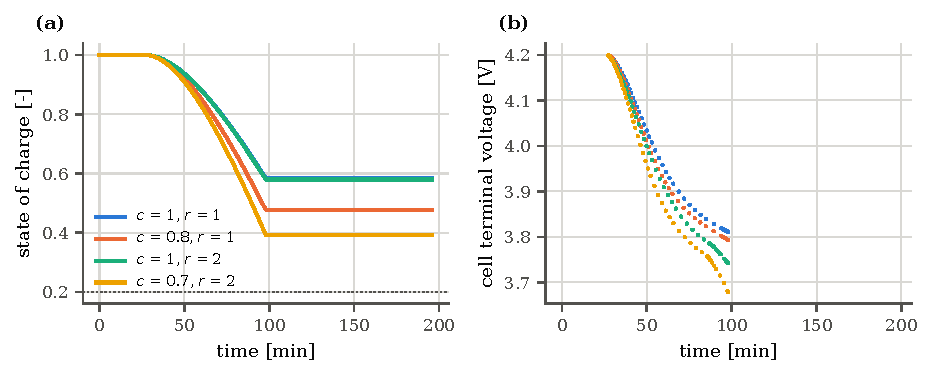
\includegraphics[width=\textwidth]{figures/fig_aged_flight.pdf}
\caption{The BOL-sized Class-II pack of \code{hybrid_config('II')} flown at 500~nm with four
states of health (capacity fraction $c$, resistance factor $r$). (a)~SOC. (b)~Cell terminal
voltage where $\varphi>0$. Script: \code{fig_class_ii_mission.py}.}
\label{fig:aged}
\end{figure}

\subsection{Post-design ground charge and cycle life}

\code{Battery.thermal_degradation_analysis} runs on a sized Class-II pack and
never enters the weight loop. It builds a \code{BatteryAgeingModel}
(\code{Systems/Battery/degradation.py}, adapted from work by Francesco Campagna according to its
docstring) and caches the result on \code{Battery.ageing} and in
\code{AircraftResults.extras['battery_ageing']}.

\emph{The cycle.} One cycle is the mission last flown by the sized pack, followed by a ground
recharge. The analysis reads it from the mission: the states $i_t^{pack}(t)$ and $T(t)$ of
\code{Mission.integral_solution}, from the start of the climb to the landing, and the state
after the taxi-in, \code{Mission.battery_end_state}. Three quantities follow.
\begin{itemize}
\item The depth of discharge. The pack starts the taxi-out full, so
  $\mathrm{DoD}=1-\mathrm{SOC}_{low}$, where $\mathrm{SOC}_{low}$ is the lowest SOC reached,
  taxi-in included.
\item The flight temperature $\bar T$, the time average of the cell temperature over the flown
  profile (trapezoidal rule). The ground legs are not part of this average.
\item The start of the recharge: the SOC and the cell temperature at the end of the taxi-in.
\end{itemize}
An explicit argument \texttt{soc\_start} sets the start of the recharge and the DoD
$\mathrm{SOC}_{max}-\mathrm{SOC}_{start}$. An explicit \texttt{flight\_temp\_k} sets the flight
temperature. Without a flown mission the defaults are $\mathrm{SOC}_{min}$ and the present
\code{Battery.T}.

\emph{Ground recharge.} A constant-current charge at the C-rate $C_{ch}$ from
$\mathrm{SOC}_{start}$ to $\mathrm{SOC}_{max}$ (default 1) lasts
$t_{ch}=60(\mathrm{SOC}_{max}-\mathrm{SOC}_{start})/C_{ch}$ minutes. The cell temperature is
stepped explicitly with $\Delta t=5$~s:
\begin{equation}
T_{k+1} = T_k + \frac{\Delta t}{C_{th}}\left(\dot q_{gen,k} - \dot q_{cp,k}\right),\qquad
\dot q_{gen,k} = (C_{ch}Q_0)^2R(T_k),\qquad
\dot q_{cp,k} = h_g A_s (T_k - T_c),
\end{equation}
with $h_g$ the \texttt{'Ground Cooling Coefficient'} (default 150~W/(m$^2$K)) and $T_c$ the
\texttt{'Coolant Temperature'} (default 20\degC). The cold-plate heat flow $\dot q_{cp}$ has two
parts. While the pack cools down ($\dot q_{cp}>\dot q_{gen}$), the cold plate rejects all the
Joule heat of the charge and, in addition, heat that the pack brought from the flight. While
the pack warms up, all of the cold-plate heat is Joule heat of the charge. The heat of the
charge rejected by the cold plate is therefore $\min(\dot q_{cp},\dot q_{gen})$, and the
remainder $\max(\dot q_{cp}-\dot q_{gen},0)$ is the pull-down of the stored flight heat. The
analysis reports the peak pack values of the two parts separately, as \code{peak_cooling_w}
and \code{peak_pulldown_w}. The first is the cooling load set by the charge rate. The second is
set mainly by the temperature at which the pack arrives. The result also reports the start and end temperatures and the peak Joule
heat \code{peak_heat_w}.

\emph{Cycle life.} The Wang et al.\ (2011) capacity-fade law, as implemented in
\code{_cycles_to_eol}, gives the charge throughput to the EOL capacity loss
$\Delta Q_{EOL}=100(1-c_{EOL})$~\% at constant C-rate $C$ and temperature $T$:
\begin{equation}
A_h = \left[\frac{\Delta Q_{EOL}}{\mathcal{A}\exp\left(\dfrac{-E_a + \mathcal{B}\,C}{\mathcal{R}T}\right)}\right]^{1/z},
\qquad N = \frac{A_h}{\mathrm{DoD}\;Q_0},
\end{equation}
with the defaults \code{WANG_DEFAULTS}: $\mathcal{A}=31\,630$, $E_a=31\,700$~J/mol,
$\mathcal{B}=370.3$, $z=0.55$, $\mathcal{R}=8.314$~J/(mol\,K). The flight (discharge C-rate,
temperature $\bar T$) and the recharge (charge C-rate, end-of-charge temperature) each give a
damage per cycle $D=s\cdot0.5/N$ with weight $s=0.25$. They add linearly (Miner) or as an $L_p$
norm when \texttt{damage\_exponent} is not 1, and the cycle life is $1/D_{total}$.

The law takes one temperature per part of the cycle. The time average $\bar T$ weights each
temperature by the time the cell spends at it. The end-of-flight temperature would instead
depend on how long the pack idled before landing, and the peak temperature is held only on the
part of the flight at the thermostat ceiling. The fade rate is convex in $T$: its Arrhenius
factor $\exp[-(E_a-\mathcal{B}C)/(\mathcal{R}T)]$ has
$(E_a-\mathcal{B}C)/\mathcal{R}=3679$~K at 3C, more than twice the cell temperature. By Jensen's
inequality the rate at $\bar T$ is therefore not larger than the time average of the rate, so
$\bar T$ gives a slightly optimistic life. On the baseline below, $\bar T=32.2$\degC, while the
temperature with the time-averaged Arrhenius factor is 33.8\degC. At a 2C charge the life is
1200 cycles with $\bar T$ and 1109 cycles with 33.8\degC.

Figure~\ref{fig:charge} shows the analysis on the Class-II baseline with a 3C discharge rate.
The flown cycle has $\mathrm{SOC}_{low}=0.204$, a DoD of 0.796, and $\bar T=32.2$\degC. The
cell flies between 20.5 and 50.0\degC. The baseline taxi draws no battery power, so the
recharge starts at the landing state, 25.9\degC. The recharge time falls from 95.5~min at 0.5C
to 11.9~min at 4C. The end-of-charge temperature rises from 20.4 to 34.9\degC, and the estimated
life falls from 1441 to 676 cycles. The peak cooling of the charge heat grows with the charge
rate, from 5.5~kW at 0.5C to 75.2~kW at 2C and 221.9~kW at 4C. Up to 2C the pack cools during
the whole charge, so this peak equals the peak Joule heat, which occurs at the coldest point.
The pull-down peak is 83.9~kW at 0.5C and 15.3~kW at 2C. From 2.5C the Joule heat exceeds the
cold-plate heat flow from the first step on, and there is no pull-down.

\begin{figure}[t]
\centering
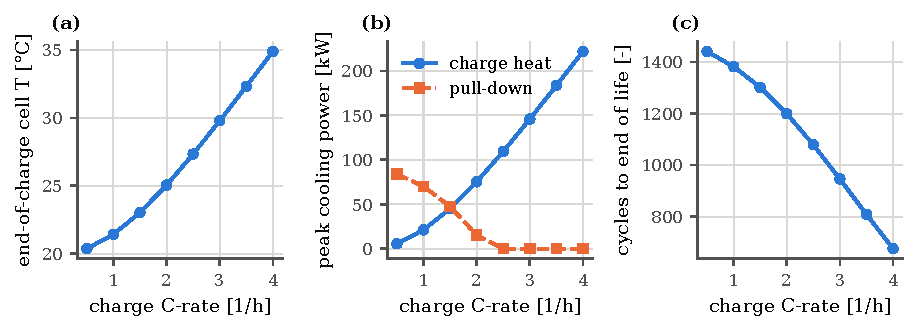
\includegraphics[width=\textwidth]{figures/fig_ground_charge.pdf}
\caption{Post-design ground fast charge of the Class-II baseline pack versus charge C-rate
(\code{thermal_degradation_analysis}, discharge C-rate 3, flown DoD and mean flight
temperature). (a)~Cell temperature at the end of the charge. (b)~Peak pack cooling power of
the charge heat and of the pull-down of the flight heat. (c)~Cycles to 80~\% capacity.
Script: \code{fig_class_ii_mission.py}.}
\label{fig:charge}
\end{figure}

\subsection{Mission-driven ageing: not implemented}

No function turns a flown mission into a state of health. The coupling design $\to$ duty cycle
$\to$ state of health $\to$ EOL design is therefore open. The Class-II mission already produces
the inputs such an estimator needs: the charge throughput $i_t^{pack}(t)$ (state $y_3$), the
current, the cell temperature $T(t)$ (state $y_4$), and the terminal and open-circuit voltages
(\code{plottingVars}). The thesis proposal in \code{thesis_proposals/hybrid-FC-battery/} plans
such an estimator based on the semi-empirical model of Schmalstieg et al.\ (J.~Power Sources
257 (2014) 325--334). That model, identified on a 2.05~Ah NMC 18650 cell, superposes calendar
and cycle ageing:
\begin{equation}
C = 1 - \alpha_{cap}(T,V)\,t^{0.75} - \beta_{cap}(\bar V,\Delta\mathrm{DOD})\sqrt{Q},\qquad
R = 1 + \alpha_{res}(T,V)\,t^{0.75} + \beta_{res}(\bar V,\Delta\mathrm{DOD})\,Q,
\end{equation}
with $t$ in days and the charge throughput $Q$ in Ah. The calendar factors are Arrhenius in
temperature and linear in voltage, $\alpha_{cap}=(7.543V-23.75)\times10^6e^{-6976/T}$ and
$\alpha_{res}=(5.270V-16.32)\times10^5e^{-5986/T}$. The cycle factors are quadratic in the mean
voltage $\bar V$ and linear in the cycle depth. All cycle tests of that paper were run at 1C and
35\degC, so the C-rate is not a model variable. A power-sized aviation pack works at much higher
C-rates, which is the main caveat for its use here.

%======================================================================
\section{Usage}
\label{sec:usage}
%======================================================================

This section shows how to set up, run and read a battery design. The snippets were run against
the code state of this manual from \code{trunk/examples}, so that \code{common} is importable.

\subsection{Designing with the typed API}

\begin{lstlisting}
import PhlyGreen as pg
from common import hybrid_config                # trunk/examples on sys.path

cfg = hybrid_config(battery_class='I')           # parallel hybrid, Class-I battery
cfg.mission.taxi_phi = 1.0                       # electric taxi
cfg.energy.battery_capacity_fraction = 0.8       # size the pack at end of life
aircraft = pg.build_aircraft()
aircraft.configure(cfg)                           # ReadInput + DesignAircraft
r = aircraft.results()
print(r.WTO, r.WBat, aircraft.weight.WBatidx)     # 23563 kg, 2207 kg, 0 (energy limited)
\end{lstlisting}

For loops and parallel studies use the pure function \code{pg.run_design(cfg)}, which deep-copies
the configuration and returns an \code{AircraftResults}. On \code{hybrid_config('I')} it returns
$W_{bat}=1542.6$~kg. A Class-II battery is defined with a \code{CellConfig}. The class, the
minimum SOC and the two temperatures are required. \code{model} defaults to
\texttt{'Finger-Cell-Thermal'}, \code{pack_voltage} to 740~V, and a \texttt{None} specific energy
or power keeps the database cell. \code{CellConfig.Ebat} and \code{CellConfig.pbat} are not read;
setting them raises a \code{DeprecationWarning}.

\begin{lstlisting}
from PhlyGreen.config import CellConfig
cfg = hybrid_config('II')
cfg.cell = CellConfig(cell_class='II', model='Finger-Cell-Thermal',
                      specific_energy=300.0, specific_power=2000.0, minimum_soc=0.2,
                      pack_voltage=800.0, initial_temperature=25.0,   # [C]
                      max_operative_temperature=50.0)                 # [C]
\end{lstlisting}

\subsection{Reading the results}

\code{AircraftResults} carries \code{WBat}, \code{battery_class}, \code{pack_energy} (in Wh), \code{pack_power_max} [W], \code{S_number} and \code{P_number}.
\code{hex_mass} is \code{Weight.WHeat_Exchanger}, which in a \texttt{'Hybrid'} is the battery
cooling mass of Eq.~\eqref{eq:hex}. \code{empty_weight} is every mass that is not payload or
fuel, so it includes the battery and the cooling mass. On \code{hybrid_config('II')} these are
20.0~kg and 15\,230~kg. The subsystems hold the rest:

\begin{lstlisting}
import numpy as np
aircraft = pg.build_aircraft(); aircraft.configure(hybrid_config('II'))
b, m, w = aircraft.battery, aircraft.mission, aircraft.weight
b.S_number, b.P_number, b.pack_weight          # 190, 110, 1483.9 kg
w.TotalEnergies                               # [fuel chemical, battery terminal] [J]
m.Max_PBat, m.TO_PBat, m.EBat_ground          # battery powers [W], ground energy [J]
m.Max_Bat_Thermal_Pwr, w.WHeat_Exchanger      # 30.1 kW, 20.0 kg
m.Max_PMotor, m.Max_PBus                      # serial sizing powers [W]
hist = np.array(m.plottingVars)               # t, SOC, Voc, Vout, i, T, Tamb, alt, mdot
m.Past_P_n                                    # P-number search history
ageing = b.thermal_degradation_analysis(charge_c_rate=2.0, discharge_c_rate=3.0)
\end{lstlisting}

\code{PhlyGreen.postprocess.mission_timeseries} returns an approximate SOC for both classes
and the battery temperature for Class II. Example \code{17_battery_thermal_and_degradation.py}
plots the in-flight temperature and the charge sweep.

\subsection{The cell model on its own}

The cell can be exercised without a design, which is how Figures~\ref{fig:discharge} and
\ref{fig:power} were made:

\begin{lstlisting}
a = pg.build_aircraft(); a.configure(cfg, design=False)   # ReadInput only
b = a.battery
b.Configure(100)                    # P = 100 parallel cells
b.T = b.Tref; b.it = 0.0            # temperature [K], drawn charge [Ah]
b.i = b.Power_2_current(200e3)      # pack current [A] for 200 kW
b.Vout, b.cell_i, b.SOC             # validated outputs
b.phi = 1.0                         # battery in use (thermostat logic)
dTdt, q_cell = b.heatLoss(288.15, 1.225)   # ambient T [K], density [kg/m^3]
\end{lstlisting}

\subsection{Aged and off-design flights}

\begin{lstlisting}
from importlib import import_module
ex30 = import_module('30_off_design_mission')       # run from trunk/examples
sized = ex30.gt_hybrid_design()
r = ex30.fly_off_design(sized, 500.0, state_of_health={'battery_capacity_fraction': 0.8})
r.feasible, r.violations, r.battery_energy_kWh, r.battery_soc_used
\end{lstlisting}

\subsection{Examples}

The battery appears in examples \code{02_hybrid_with_battery.py}, \code{02b_serial_hybrid.py},
\code{15_class_i_vs_class_ii.py}, \code{16_class_ii_propulsion_sizing.py},
\code{17_battery_thermal_and_degradation.py}, \code{18_serial_range_extender_gt.py},
\code{23_fuelcell_battery_hybrid.py}, \code{25_fuelcell_battery_class_ii_models.py} and
\code{30_off_design_mission.py}. The index is \code{trunk/examples/README.md}.

\subsection{Pitfalls}

\begin{itemize}
\item \emph{Run time.} A Class-II design repeats the whole mission for every evaluated $P$. The
  baseline needs 41 mission evaluations and between 17 and 26~s; a Class-I design takes 1.6 to 2.4~s. Sweeps
  with Class II should be planned accordingly, and the \code{pg.run_design} function can be
  parallelized.
\item \emph{Infeasible packs.} When no pack lighter than the aircraft flies the mission, the
  P-number search raises \code{PACK_HEAVIER_THAN_AIRCRAFT} (Section~\ref{sec:psearch}). With a
  specific energy of 20~Wh/kg, \code{hybrid_config('II')} flown at $W_{TO}=21\,630$~kg evaluates
  $P=64$, 128, 256, 512, 1024 and $P_{lim}=1603$. The pack of 1603 strings still violates the
  SOC limit, so the search raises.
\item \emph{The ``rtol may be too loose'' warning} means that a stored output point violated a
  limit that the integration itself respected. It does not change the design. The baseline
  run printed none.
\item \emph{No margin at the design point.} The sized pack ends the design mission at
  $\mathrm{SOC}_{min}$ within one string. Any degradation or a longer mission makes it
  infeasible. Size at EOL if the aged aircraft must fly the design mission.
\item \emph{Meaning of $\varphi$.} The same input means a supplied-power share in
  \texttt{'Hybrid'} and a propulsive-power share in \texttt{'FuelCellBattery'}
  (Section~\ref{sec:phi}).
\item \emph{Specific energy of the examples.} \code{hybrid_config} uses 1500~Wh/kg. Results
  scale strongly with this input.
\end{itemize}

%======================================================================
\section{Verification and limitations}
\label{sec:verification}
%======================================================================

This section lists the tests that pin the battery behaviour and the assumptions and
limitations of the model.

\subsection{Tests}

The suite runs from \code{trunk/} with \code{pytest} (\code{-m "not slow"} for the fast part).
Table~\ref{tab:tests} lists the tests that involve the battery.

\begin{table}[h]
\centering\small
\caption{Tests that pin battery behaviour (\code{trunk/tests/}).}
\label{tab:tests}
\begin{tabular}{@{}p{5.4cm}p{9.4cm}@{}}
\toprule
File & What is pinned\\
\midrule
\code{regression/test_golden_design.py} & Golden master of the tutorial Class-II parallel hybrid (\code{golden/hybrid_parallel_atr.json}, $W_{TO}=23\,547.1$~kg): \code{WBat}, \code{pack_energy}, \code{pack_power_max}, \code{SourceEnergy} and $\Psi$, with the general mass and power fields, to a relative tolerance of $10^{-4}$.\\
\code{regression/test_weight_sizing.py} & The Class-II battery cooling mass is positive and enters $W_{TO}$.\\
\code{regression/test_ground_segments.py} & Taxi/take-off split inputs and validation; fuel taxi draws no battery; electric taxi moves ground energy to the battery and into \code{Max_PBat}; $\varphi_{taxi}$ defaults to $\varphi_{TO}$; \code{takeoff_power_fraction}; fuel-cell electric taxi; a Class-II pack starts the climb with charge drawn.\\
\code{regression/test_degradation.py} & Class-I and Class-II \code{set_state_of_health} scaling and reset; EOL sizing enlarges the pack.\\
\code{unit/test_battery_degradation.py} & Ground recharge time, cooling and temperature are physical; faster charge needs more cooling; cycle life decreases with temperature; zero C-rate gives infinite time.\\
\code{unit/test_battery_cell.py} & Cell voltage model against the Shepherd equation and its trends; \code{Power_2_current} round trip with the power, zero power and no solution; \code{heatLoss} (Bernardi heat, adiabatic below the ceiling, idle cooling); rescaling to a target specific energy and power; series count; \code{find_parallel_cells} on monotone stubs, warm starts and the \code{PACK_HEAVIER_THAN_AIRCRAFT} bound.\\
\code{regression/test_battery_sizing_analysis.py} & Cycle life on the flown DoD and the mean flight temperature, independent of \code{Battery.T}; explicit overrides; the ground-charge cooling peak is charge heat only and grows with the C-rate; the P-number search stops at the aircraft mass; the serial generator specific power and its default.\\
\code{regression/test_off_design.py} & \code{fly_off_design} reproduces the design and flags limits on a GT hybrid.\\
\code{regression/test_fuelcell_battery.py} & FC+battery closes; no battery at $\varphi=0$; more $\varphi$ grows the battery; the Class-II pack is P-number sized and carries a cooling mass; the motor and PMAD are sized on the drive peak \code{Max_PDrive}.\\
\code{regression/test_fc_battery_takeoff_assist.py} & When a take-off battery pays on a fuel-cell aircraft: never on the baseline field, where the climb sizes the stack; on an 800~m field it shrinks the stack, does not pay with the default pack, and pays with an assumed 3~kW/kg pack on the take-off run only.\\
\code{regression/test_tms_design.py} & FC+battery Class II at $\varphi=0$ matches the hydrogen design.\\
\code{unit/test_powertrain_graph.py}, \code{regression/test_powertrain_equivalence.py} & Graph power ratios, including $\Pi_5$, equal the legacy matrices.\\
\code{regression/test_class_ii_sizing.py} & Gas-turbine and motor nominal-power checks (\code{report_class_ii_sizing}); not the battery itself.\\
\bottomrule
\end{tabular}
\end{table}

\subsection{Modelling assumptions and limitations}

\begin{itemize}
\item One representative cell; all cells share current, temperature and state of charge. No
  cell-to-cell spread, balancing or string failure.
\item Pack mass and volume are cell mass and a simple stacking; no module, enclosure, wiring or
  battery-management mass. The cooling mass is the single specific-power term of
  Eq.~\eqref{eq:hex}, with no geometry of the heat exchanger or of the air duct.
\item Discharge only in flight for the phi-split paths ($\varphi\ge0$). In-flight recharge exists
  only in the range extender, which uses the Class-I model.
\item Single-node thermal model with assumed $C_{th}$, $R_{i,th}$ and cooling law; an ideal
  thermostat holds the ceiling and its power is the cooling sizing load. The value of
  $R_{i,th}$ is uncited (Section~\ref{sec:thermal}).
\item The P-number search assumes that feasibility is monotone in $P$, and it accepts no pack
  heavier than the aircraft.
\item Cells beyond present technology are obtained by rescaling a database cell, keeping its
  voltage shape and its mass.
\item Ageing enters only as a prescribed state of health. The cycle-life analysis is
  post-design: it takes the mission last flown by the sized pack as one cycle, with its
  flown DoD and its time-averaged flight temperature, and it does not feed a state of health back into the
  design (Section~\ref{sec:soh}).
\end{itemize}

%======================================================================
\appendix
\section{Input reference}
\label{app:inputs}
%======================================================================

Table~\ref{tab:inputs} lists the inputs that act on the battery. ``req.'' means that the code
reads the key without a default.

\small
\begin{longtable}{@{}p{3.6cm}p{3.6cm}p{1.5cm}p{1.5cm}p{3.9cm}@{}}
\caption{Battery inputs: typed field, legacy dictionary key, default, unit and meaning. The
baselines of \code{examples/common.py} write the ground-segment inputs, the state of health, the
battery cooling specific power, the generator specific power and the post-design analysis
fields explicitly at these defaults.}
\label{tab:inputs}\\
\toprule
Typed field & Legacy key & Default & Unit & Meaning\\
\midrule
\endfirsthead
\toprule
Typed field & Legacy key & Default & Unit & Meaning\\
\midrule
\endhead
\multicolumn{5}{@{}l}{\emph{\code{CellConfig} (\texttt{CellInput})}}\\
\code{cell_class} & \texttt{Class} & req. & -- & \texttt{'I'} or \texttt{'II'}\\
\code{model} & \texttt{Model} & see text & -- & key of \code{Cell_Models} (Class II); default \texttt{Finger-Cell-Thermal}\\
\code{specific_energy} & \texttt{SpecificEnergy} & req. (I) & Wh/kg & Class I energy; Class II rescaling target, optional (unset keeps the database cell)\\
\code{specific_power} & \texttt{SpecificPower} & req. (I) & W/kg & Class I power; Class II rescaling target, optional\\
\code{minimum_soc} & \texttt{Minimum SOC} & req. & -- & lower SOC limit\\
\code{pack_voltage} & \texttt{Pack Voltage} & 740 & V & sets $S=\lfloor V_{pack}/V_{max}\rfloor$ (Class II)\\
\code{initial_temperature} & \texttt{Initial temperature} & req. (II) & \degC & cell temperature at taxi-out\\
\code{max_operative_temperature} & \texttt{Max operative temperature} & req. (II) & \degC & thermostat ceiling $T_{lim}$\\
\code{charge_c_rate} & \texttt{Charge C-Rate} & none & h$^{-1}$ & ground fast-charge rate (post-design)\\
\code{discharge_c_rate} & \texttt{Discharge C-Rate} & charge rate & h$^{-1}$ & flight rate for cycle life\\
\code{maximum_soc} & \texttt{Maximum SOC} & 1.0 & -- & SOC at the end of the charge\\
\code{eol_capacity} & \texttt{EoL Capacity} & 0.8 & -- & EOL capacity fraction for cycle life\\
\code{coolant_temperature} & \texttt{Coolant Temperature} & 20 & \degC & ground coolant inlet\\
\code{ground_cooling_coefficient} & \texttt{Ground Cooling Coefficient} & 150 & W/(m$^2$K) & ground cold plate $h_g$\\
\code{Ebat}, \code{pbat} & \texttt{Ebat}, \texttt{pbat} & -- & -- & not read; setting them raises a \code{DeprecationWarning}\\
\midrule
\multicolumn{5}{@{}l}{\emph{\code{EnergyConfig} (\texttt{EnergyInput})}}\\
\code{battery_capacity_fraction} & \texttt{Battery Capacity Fraction} & 1.0 & -- & state of health $c$\\
\code{battery_resistance_factor} & \texttt{Battery Resistance Factor} & 1.0 & -- & state of health $r$\\
\code{battery_specific_energy} & \texttt{Battery Specific Energy} & 250 & Wh/kg & FC+battery Class I\\
\code{battery_specific_power} & \texttt{Battery Specific Power} & 1500 & W/kg & FC+battery Class I\\
\code{battery_usable_soc} & \texttt{Battery Usable SOC} & 0.8 & -- & FC+battery Class I usable fraction\\
\code{hex_specific_power_battery} & \texttt{HEX Specific Power Battery} & 1500 & W/kg & battery cooling, Eq.~\eqref{eq:hex}\\
\code{gt_rated_power} & \texttt{GT Rated Power} & none & W & enables the range extender\\
\code{battery_charge_efficiency} & \texttt{Battery Charge Efficiency} & 1.0 & -- & range-extender recharge\\
\code{eta_electric_motor} & \texttt{Eta Electric Motor} & req. & -- & parallel motor\\
\code{eta_electric_motor_1}, \code{_2} & \texttt{Eta Electric Motor 1}, \texttt{2} & req. (serial) & -- & generator, motor\\
\code{eta_pmad} & \texttt{Eta PMAD} & req. & -- & power management\\
\code{specific_power_powertrain} & \texttt{Specific Power Powertrain} & req. & W/kg & [thermal, electric motor]\\
\code{specific_power_pmad} & \texttt{Specific Power PMAD} & 10000 & W/kg & PMAD mass\\
\code{specific_power_generator} & \texttt{Specific Power Generator} & $p_{em}$ & W/kg & serial generator mass\\
\midrule
\multicolumn{5}{@{}l}{\emph{\code{MissionConfig} (\texttt{MissionInput}) and stages}}\\
\code{taxi_phi} & \texttt{Taxi Supplied Power Ratio} & $\varphi_{TO}$ & -- & battery share of taxi\\
\code{taxi_out_time}, \code{taxi_in_time} & \texttt{Taxi Out Time}, \texttt{Taxi In Time} & 13, 13 & min & taxi durations\\
\code{taxi_power_fraction} & \texttt{Taxi Power Fraction} & 0.07 & -- & of the take-off power\\
\code{takeoff_time} & \texttt{Takeoff Time} & 0.7 & min & take-off run\\
\code{takeoff_power_fraction} & \texttt{Takeoff Power Fraction} & 1.0 & -- & of the take-off power\\
\code{Segment(phi=...)} & \texttt{Supplied Power Ratio: phi} & 0 & -- & constant $\varphi$ (and $\varphi_{TO}$)\\
\code{Segment(phi_start, phi_end)} & \texttt{phi\_start}, \texttt{phi\_end} & 0, 0 & -- & linear $\varphi$ ramp\\
\midrule
\multicolumn{5}{@{}l}{\emph{\code{WellToTankConfig}, \code{ClimateImpactConfig}}}\\
\code{eta_charge} & \texttt{Eta Charge} & 1.0 & -- & charger efficiency (well-to-wake)\\
\code{eta_grid} & \texttt{Eta Grid} & 1.0 & -- & grid efficiency\\
\code{grid_co2} & \texttt{Grid\_CO2} & req. if $E_b>0$ & kg/MJ & grid CO$_2$ intensity\\
\bottomrule
\end{longtable}
\normalsize

Instance attributes that are not inputs but change the behaviour: \code{Mission.size_battery_pack}
(default \texttt{True}), \code{Mission.optimal_n} and \code{Mission.last_weight} (search warm
start), and \code{Battery.pack_Vmax}.

\section{Reproducing the figures}

\begin{lstlisting}[language=bash]
conda run -n phlygreen python manuals/battery/scripts/make_figures.py
cd manuals/battery && latexmk -pdf -interaction=nonstopmode -outdir=build battery_manual.tex
\end{lstlisting}
The driver runs \code{fig_cell.py}, \code{fig_class_ii_mission.py} and
\code{fig_sizing_studies.py}. It takes about five minutes, most of it in the Class-II designs.

\end{document}
